% This package warns you for incorrect usage of \Latex
% The warnings show up in the .log file
\RequirePackage[12tabu, orthodox]{nag}
\documentclass[a4paper]{report}

%%%%%%%%%%%%%%%%%%
%    PACKAGES
%%%%%%%%%%%%%%%%%%
\usepackage[utf8]{inputenc}
\usepackage[T1]{fontenc}
\usepackage[french]{babel}
\usepackage{lmodern}

\usepackage{geometry}        % Gestion des marges
% Options : twoside, landscape, portrait; textwidth, textheight, text; [t|b|r|l]margin
\usepackage{graphicx, xcolor, titling, titlesec, titletoc, makeidx, fancyhdr, enumitem, array, diagbox, subfigure, algorithm, algorithmic, placeins, comment}
\usepackage{amsmath, amssymb, mathrsfs, amsthm, mathtools, mathdots}
\usepackage{hyperref}
%%%%%%%%%%%%%%%%%%%%%%%%%%%%%%%%%%%%%%%%%%%%%%%%%%%%%%%%%%%%%%%%%%%



%\input  : se contente d'un copier / coller
%\include : ajout d'un saut de page
%\includeonly{fichier1 ...}
%%%%%%%%%%%%%%%%%%%%
% FILE : COMMANDES
%\newcommand\nomCommande[nbArgument][ValeurParDef]{CodeLatex}
% #i est le nom de la ieme variable. i <= 9. Valeur par défaut
% appel de la commande : \nomCommande{arg1}{arg2}
% package xargs permet de s'affranchir de la limite du nombre de paramètre

%%%%%%%%%%%%%%%%%%%
% 1. Theorem
%%%%%%%%%%%%%%%%%%%
\newtheorem{definition}{Définition}
\newtheorem{theoreme}{Théorème}
\newtheorem{preuve}{Preuve}
\newtheorem{propriete}{Propriété}
\newtheorem{corollaire}{Corollaire}
\newtheorem{ex}{Exemple}
\newtheorem{remarque}{Remarques}
% utilisation via : \begin{definition} ... \end{definition}
%%%%%%%%%%%%%%%%%%%%%


%%%%%%%%%%%%%%%%%%%
% 2. Commandes
%%%%%%%%%%%%%%%%%%%
% Commandes Latex pour les mathématiques
\newcommand\grandO[1]{\ensuremath{O\mathopen{}\left(#1\right)}}

\newcommand{\fonction}[5]{\begin{array}{l|ccl}
#1: & #2 & \longrightarrow & #3 \\
    & #4 & \longmapsto & #5 \end{array}}
    
\newcommand{\intervalle}[4]{\ensuremath{\mathopen{#1}#2\mathclose{}\mathpunct{};#3\mathclose{#4}}}
\newcommand{\intervalleff}[2]{\intervalle{[}{#1}{#2}{]}}
\newcommand{\intervalleof}[2]{\intervalle{]}{#1}{#2}{]}}
\newcommand{\intervallefo}[2]{\intervalle{[}{#1}{#2}{[}}
\newcommand{\intervalleoo}[2]{\intervalle{]}{#1}{#2}{[}}
\newcommand{\intervalleentier}[2]{\intervalle\llbracket{#1}{#2}\rrbracket}

\newcommand{\infini}{\ensuremath{O}}
\newcommand{\ensnombre}[1]{\ensuremath{\mathbb{#1}}}
\newcommand{\N}{\ensnombre{N}}
\newcommand{\Z}{\ensnombre{Z}}
\newcommand{\Q}{\ensnombre{Q}}
\newcommand{\R}{\ensnombre{R}}
\newcommand{\C}{\ensnombre{C}}
\newcommand{\field}[1][K]{\ensnombre{#1}}
\newcommand{\GF}[1]{\ensuremath{\ensnombre{F}_{#1}}}
\newcommand{\Zn}[1]{\ensuremath{\Z/#1\Z}}
%\frac{\Z}{#1\Z}}}
\newcommand{\closure}[1][\ensnombre{K}]{\ensuremath{\overline{#1}}}
\newcommand{\CE}[1][\closure]{\ensuremath{E(#1)}}

\newcommand{\abs}[1]{\left\lvert#1\right\rvert}
\newcommand{\norme}[1]{\left\lVert#1\right\rVert}

\newcommand{\enstq}[2]{\left\{#1\mathrel{}\middle|\mathrel{}#2\right\}}

\newcommand{\prodscal}[2]{\left\langle#1,#2\right\rangle}

\DeclareMathOperator*{\argmin}{arg\,min}

\newcommand{\todo}[1]{\textcolor{red}{#1}}

%%%%%%%%%%%%%%%%%%%%
% FILE : NOMENCLATURE
%\input{nomenclature}


% Infos page de titre
\title{Notes sur les Courbes Elliptiques}
\author{Maxime \textsc{Lebreton}} %\and si plusieurs auteurs
\date{\today}


\begin{document}
\maketitle
\newpage
\tableofcontents
\newpage
%\begin{abstract}
%\end{abstract}
%\newpage
%\printnomenclature
%\newpage
%\listoftables
%\listoffigures

% MEMO Clavier MAC
% antislash : Alt + Maj + / 
% accolade : Alt + (
% crochet Alt + Maj + (
% underscore : Maj + -
% barre vertical : Alt + Maj + l


\addtolength{\parskip}{1em}


\chapter{Questions, Todo List}

\section{Questions}
\begin{itemize}[label=--]
    \item Quelle est la différence entre un isomorphisme sur \field{}, une isogénie sur \field{} et une équivalence birationnelle \field{} ? Les trois notions sont des relations d'équivalence mais de plus en plus faible, c'est à dire que le nombre de classes d'équivalence est de moins en moins grand. Un isomorphisme est une isogénie qui elle-même est une équivalence birationnelle. Les réciproques sont fausses. On les considère uniquement définies sur \GF{p} car sinon elles sont cryptographiquement différentes. 
    \item L'algorithme de Montgomery ladder est-il adapté aux SM à bases multiples ? Si non pourquoi.
    \item \'A quelle condition une courbe d'Edwards peut-elle être transformée en une tordue d'Edwards avec $a=-1$ ? Même question mais en partant d'une tordue d'Edwards avec $a\neq-1$.
    \item Discriminant du corps des endomorphismes. S'il est faible, qu'est-ce que cela signifie : qu'il possède un endomorphisme facilement calculable ?
    \item \'Ecriture générique d'une isogénie (cf. Benjamin Smith).
\end{itemize}


\section{Remarques}



\section{Si j'ai le temps}
\begin{itemize}[label=--]
    \item \'Etude du théorème de Rieman-Roch.
    \item Discriminant d'un polynôme.
    \item Dérivées partielles, implicites.
\end{itemize}

\chapter{Introduction aux courbes elliptiques}
\section{Généralités}
\subsection{Définitions}
\begin{definition}
Une équation de Weierstrass affine généralisée d'une courbe elliptique $E$ sur \field{} est donnée par :
\begin{equation}
y^2 + a_1 xy + a_3 y = x_3 + a_2x^2 + a_4x + a_6
\end{equation}
\begin{equation}
f(x, y) = y^2 + a_1 xy + a_3 y - x_3 - a_2x^2 - a_4x - a_6
\end{equation}
avec $a_1, a_2, a_3, a_4, a_5, a_6  \in \field{}$ et $\Delta \neq 0$ où $\Delta$ est le discriminant de $E$ et est défini de la façon suivante : 
\begin{equation}
\begin{cases}
\Delta & = -b_2^2 b_8 - 8b_4^3 - 27b_6^2 + 9 b_2b_4b_6\\
b_2 &= a_1^2 + 4a_2,\\
b_4 &= 2a_4 + a_1a_3\\
b_8 &= a_1^2a_6 + 4a_2a_6 - a_1a_3a_4 + a_2a_3^2 - a_4^2
\end{cases}
\end{equation}
\end{definition}

\vspace{0.5cm}

\begin{itemize}[label=--]
    \item Une courbe elliptique consiste à l'ensemble des zéros d'un polynôme à deux variables de degré trois de la forme précédente auquel on adjoint un point à l'infini. C'est une courbe plane algébrique.
    \item La condition $\Delta \neq 0$ assure (et réciproquement) que la courbe $E$ ne possède aucun point singulier à coordonnées dans \closure{} \footnote{Les coordonnées des points sont automatiquement algébriques.}, c'est à dire de points dont les dérivées partielles s'annulent. Si $f(x_1, y_1) = 0$ avec $(x_1, y_1) \in \closure{}^2$, alors le vecteur $\left (\frac{\delta P}{\delta x}(x_1, y_1), \frac{\delta P}{\delta y}(x_1, y_1) \right )$ n'est pas le vecteur nul. On parle alors de courbe \emph{non singulière} ou \emph{lisse}. Cette équivalence se vérifie sans peine. 
    \item Un point de la courbe est non singulier s'il admet une unique tangente en ce point. Cela se traduit par l'absence de racines multiples\footnote{La nullité du discriminant d'un polynôme équivaut à la présence de racines multiples dans son corps de décomposition.}. La figure \ref{fig:EC} représente les graphes de courbes elliptiques à valeurs dans le corps des réels et un corps fini.
\end{itemize}

\begin{definition}
Soit $\field{} \hookrightarrow \field[L]$ une extension de corps. Il est possible de s'intéresser à l'ensemble des points de la courbe $E/\field{}$ dans n'importe quelle extension algébrique de \field{}. On parle des points \field[L]-rationnels de $E/\field{}$. Lorsque rien n'est précisé, on considère implicitement la clôture algébrique de $\closure{}$, $E(\closure{})$.
\begin{equation}
    E(\field[L]) = \{(x,y) \in \field[L]^2\ \mid\ f(x,y) = 0\} \cup \{O\}
\end{equation}
Le corps \field[L] est appelé \emph{corps des points rationnels}\footnote{Ground field.}. Qu'il ne faut pas confondre avec le corps de base\footnote{Base Field.} \field{} qui est le plus petit corps contenant les coefficients de l'équation.
\end{definition}

\begin{figure}[ht]
\centering
    \subfigure[Courbes elliptiques sur \R]
    {
       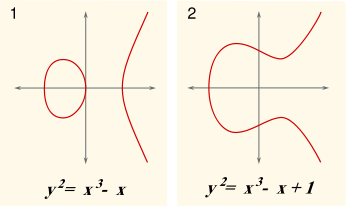
\includegraphics[scale=0.6]{images/EC_R.png}
       \label{fig:ECR}
     }
     \subfigure[Courbe elliptique sur un corps fini]
     {
       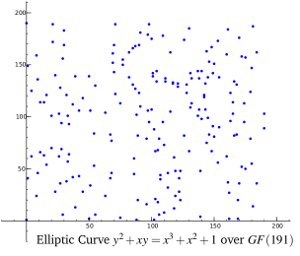
\includegraphics[scale=0.5]{images/EC_ff.png}
       \label{fig:ECFF}
     }
    \label{fig:EC}
    \caption{Graph de courbes elliptiques}
\end{figure}

\vspace{0.5cm}
Quelques rappels sur l'\emph{espace projectif} s'impose. C'est une construction qui permet d'homogénéiser un espace vectoriel, autrement dit d'oublier les proportionnalités pour ne plus considérer que les directions.
\begin{definition}
Soit $E$ un \field{}-espace vectoriel. L'\emph{espace projectif} déduit de $E$ et noté \ensnombre{P}$(E)$  est l'ensemble des droites vectorielles de $E$.

En d'autres termes, si $\mathcal{R}$ est la relation d'équivalence \og être proportionnel \fg{} sur $E\backslash \{0\}$ définie par $x\mathcal{R}y$ si et seulement si il existe $\lambda \in \field{}^*$ tel que $x = \lambda y$, alors $\ensnombre{P}(E) = (E \backslash \{0\}) /_{\mathcal{R}}$.

Une classe d'équivalence, noté $[X_1 : \ldots : X_n]$, est appelé \emph{coordonnée homogène}. Chacune de ces classes correspond à une droite vectorielle privée de zéro. Par définition, pour tout $\lambda \in \field{}^*$, $[X_1 : \ldots : X_n] = [\lambda X_1 : \ldots : \lambda X_n]$.

Les points tels que $X_n = 0$ sont appelés \emph{points à l'infini}.

Si $E = \field{}^n$, on note \ensnombre{P}$(E) = \ensnombre{P}^n(\field{})$, l'espace projectif de dimension $n$. $\ensnombre{P}^1(\field{})$ est la droite projective et $\ensnombre{P}^2(\field{})$ est le plan projectif.

$\ensnombre{P}^n(\field{}) \simeq \ensnombre{A}^n(\field{}) \times \ensnombre{P}^{n-1}(\field{})$
\end{definition}

Citons deux articles intéressant du site Images des Mathématiques sur l'espace projectif : \href{http://images.math.cnrs.fr/L-infini-est-une-droite-comme-les.html}{Art 1}, \href{http://images.math.cnrs.fr/Et-si-on-rajoutait-une-droite-a-l.html}{Art 2}.

\begin{figure}[ht]
    \centering
    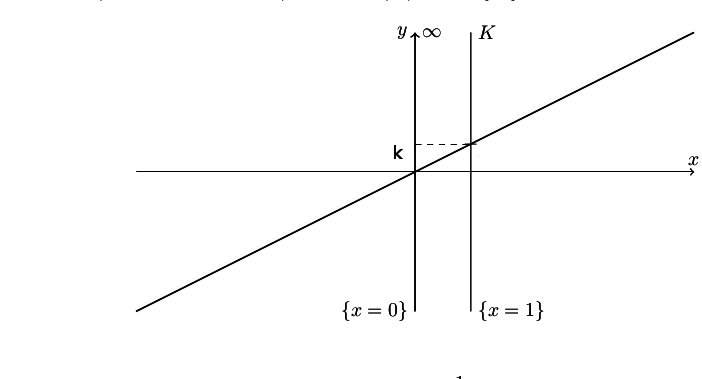
\includegraphics[scale=0.4]{images/projectif.png}
    \caption{La droite projective s'identifie à l'espace affine de dimension un auquel on ajoute un point à l'infini}
    \label{fig:projectif}
\end{figure}

\begin{definition}
Une équation de Weierstrass généralisée projective d'une courbe elliptique $E$ sur un corps \field{} est donnée par :
\begin{equation}
E : Y^2Z + a_1XYZ + a_3YZ^2 = X^3 + a_2X^2Z + a_4XZ^2 + a_6Z^3
\end{equation}
avec $a_1, a_2, a_3, a_4, a_5, a_6  \in \field{}$ et $\Delta \neq 0$.
\end{definition}

\begin{itemize}[label = --]
    \item Soit $f(x,y) = 0$ une courbe affine. On obtient sa version projective en définissant la courbe $\tilde{f}(x,y,z) = 0$ où $\tilde{f}$ est le polynôme homogène associé à $f$. $\tilde{f}(x,y,z) = z^n f(x,y)$ et $\tilde{f}(x,y,1) = f(x,y)$.
    \item Le point à l'infini, noté \infini{}, correspond à $[0 : 1 : 0]$.
    \item On peut montrer que le point à l'infini est non singulier.
\end{itemize}

\vspace{0.3cm}

Nous n'avons pas pour le moment défini ce qu'est une courbe elliptique. Nous nous sommes contentés de donner une équation de cet objet. L'équation de Weierstrass est une incarnation (générique) possible d'une courbe elliptique. Mais il en existe d'autre que nous verrons ultérieurement (forme d'Edwards, Hessienne, de Montgomery, de Legendre \ldots ). L'équivalence des définitions se démontrent à l'aide du théorème de Riemann-Roch.

\begin{definition}
Une courbe elliptique $E$ sur un corps \field{} est une courbe algébrique projective non singulière de genre $1$ avec la donnée d'un point \field{}-rationnel \infini{}.
\end{definition}

\subsection{Isomorphismes}
Finalement la donnée d'une courbe elliptique correspond à la donnée du corps de base \field{} et des coefficients $a_1, \ldots, a_6$ régissant son équation de Weierstrass. C'est ce qu'on appelle les \emph{paramètres}\footnote{Domain parameter.} d'une courbe elliptique. Dans le cadre de la cryptographie, on ajoute aussi le point de base $P$, l'ordre $l$ de ce point, ainsi que le cofacteur $h$. 

Via un changement de variables adapté, c'est à dire préservant l'équation de Weierstrass, il est possible d'obtenir une équation de Weierstrass dites réduite. En effet, si la caractéristique du corps \field{} est différente de $2$ alors l'équation se simplifie via l'application : $y \mapsto y + a_1x/2 + a_3 /2$. De même, lorsque la caractéristique du corps de base est cette fois différente de $3$, on utilise le changement de variables : $x \mapsto x + a_2/3$. Enfin, en caractéristique strictement supérieur à $3$, l'équation réduite est appelée emph{équation de Weierstrass simplifiée}\footnote{Short Weierstrass Form.}. Le tableau \ref{tab:weierstrass} résume la situation.

\begin{comment}
\begin{figure}[h]
\centering
    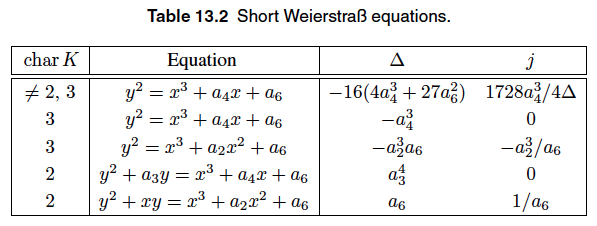
\includegraphics[scale=0.5]{images/equationWeierstrass.png}
    \caption{Equation de Weierstrass}
    \label{fig:weierstrass}
\end{figure}
\end{comment}

\begin{table}[ht]
\centering
\begin{tabular}{|c|c|cc|}
\hline
char \field{} & Equation & $\Delta$ & $j$  \\
\hline \hline
\rule[0ex]{0pt}{3ex}
$\neq 2, 3$ & $y^2 = x^3 + ax + b$ & $-16(4a^3 + 27b^2)$ & $1728 \ 4 a^3 / \Delta$\\
3 & $y^2 = x^3 + ax + b$ & $-a^3$ & 0 \\
3 & $y^2 = x^3 + a_2x^2 + a_6$ & $-a_2^3a_6$ & $-a_2^3/a_6$\\
2 & $y^2 + a_3y = x^3 + a_4x + a_6$ & $a_3^4$ & $0$ \\
2 & $y^2 + xy = x^3 + a_2x^2 + a_6$ & $a_6$ & $1/a_6$\\
\hline
\end{tabular}
\caption{\'Equation de Weierstrass en fonction de la caractéristique du corps}
\label{tab:weierstrass}
\end{table}

\todo{Comment calculer le discriminant ? }

Les seuls changement de variables admissibles sont des transformations affines dont la forme est précisé ci-après \eqref{admissibleChangeVar}. On les qualifie d'\emph{isomorphisme de courbes elliptiques}. Rappelons qu'intuitivement un isomorphisme ne correspond ni plus ni moins à un renommage des éléments. Deux courbes elliptiques isomorphes sur leur corps de base sont identiques, ou plus exactement indistinguables en tant que courbes. Elles partagent les mêmes propriétés et la même structure. L'unique différence réside dans le nom que l'on attribue aux différents points, comme un clone qui se distinguerait de son original uniquement par son nom. Définir un isomorphisme, c'est associer à chaque point son clone. 

\begin{definition}
Deux courbes elliptiques $E_1, E_2$ définies sur \field{} sont isomorphes sur \field{L}, une extension \field{}, s'il existe $u, r, s, t \in \field{L}$ et $u \ne 0$ tel que le changement de variables suivant
\begin{equation*}
    (x, y) \mapsto (u^2x + r, u^3y + u^2sx + t)
    \label{admissibleChangeVar}
\end{equation*}
transforme l'équation de Weierstrass $E_1$ en l'équation de Weierstrass de $E_2$. Cet isomorphisme définit une bijection entre l'ensemble des points $\field{L}$-rationnels (et non $\field{K}$-rationnels) de $E_1$ et ceux de $E_2$. Nous verrons que cette affirmation reste vraie pour toute extension de degré pair de $\field{L}$.
\end{definition}

% A mettre en remarque.
La structure de groupe est préservée.\\
La loi de groupe est défini par : trois points $P, Q, R$ sont alignés si et seulement si $P + Q + R = \infini{}$. 
Une isogénie de degré $1$ est un isomorphisme. Ainsi l'application précédente est bien un isomorphisme et un morphisme de groupe. On peut aussi le voir d'une autre façon. La loi de groupe est définie par le fait que les points $P, Q, R$ sont alignés si et seulement si $P + Q + R = \infini{}$. De plus dire que notre isomorphisme préserve la structure de groupe c'est dire exactement que si $P, Q, R$ sont alignés alors $\phi(P), \phi(Q), \phi(R)$ sont alignés. Ou en d'autres termes que l'image d'une droite est encore une droite. Or un changement de variables admissibles est une transformation affine et par définition elle envoie une droite sur une autre droite.

\vspace{0.2cm}

\begin{propriete}
Lorsque $char(\field{}) \geq 5$, alors deux courbes elliptiques $E_{(a, b)},\ E_{(a^{'}, b^{'})}$ sont isomorphes sur \field{} si et seulement si il existe $u \in \field{}^{*}$ tel que $(x, y) \mapsto (u^2x, u^3y)$ si et seulement si il existe $u \in \field{}^{*}$ tel que $a = u^4 a^{'}$ et $b = u^6 b^{'}$.
\end{propriete}

\begin{theoreme}
\^Etre isomorphe est une relation d'équivalence sur l'ensemble des courbes défini sur \GF{q}. Ce qui nous intéresse, n'est pas de savoir le nombre de courbes mais plutôt le nombre de classes d'isomorphisme (ie : le nombre de familles de courbes réellement distinctes)\footnote{Une classe d'isomorphisme contient un ensemble de courbes. Bien qu'elles possèdent chacune une équation qui leur est propre, structurellement elles sont identiques. Ce sont les mêmes courbes mais avec des noms différents.}. Le nombre de classes d'isomorphisme sur \GF{q} est $2q + 6$, $2q + 2$, $2q + 4$, $2q$ pour $ q \equiv 1, 5, 7, 11 \pmod{12}$.\begin{proof}
Au total il y a $q(q-1)$ courbes elliptiques (il faut que le discriminant soit non nul). Certaines courbes sont isomorphes entre elles. Trois cas disjoints sont à distinguer : $(a, 0)$, $(0, b)$ et $(a, b)$ avec dans chaque cas $a$ et $b$ non nuls. 
\begin{enumerate}
    \item $(a, 0)$ avec $a \neq 0$. Il existe $q-1$ courbes de cette forme. $Cl(a, 0) = \{ (u^4a, 0) \mid u \in \GF{q}^* \}$. Ainsi $\# Cl(a, 0) = (q-1)/(2 \text{ ou } 4)$. En fait, on a $\# Cl(a, 0) = (q-1)/ \# Aut(E)$.
    \item $(0, b)$ avec $b \neq 0$. Il existe $q-1$ courbes de cette forme. $Cl(0, b) = \{ (0, u^6 b) \mid u \in \GF{q}^* \}$. Ainsi $\# Cl(0, b) = (q-1)/(2 \text{ ou } 6)$.
    \item $(a, b)$ avec $ab \neq 0$. Il existe $(q-1)(q-2)$ courbes de cette forme. $Cl(a, b) = \{ (u^4a, u^6b) \mid u \in \GF{q}^* \}$. Ainsi $\# Cl(a, b) = (q-1)/2$.
\end{enumerate}
Finalement, le nombre de classes dépend de l'existence ou non d'un élément d'ordre $3$ (ie : si $3 \mid q-1$) et d'un élément d'ordre $4$ (ie : si $4 \mid q-1$ car $\GF{}^*$ est un groupe cyclique).
\end{proof}
Ce qu'il faut retenir est qu'il existe environ $2q$ courbes définies sur \GF{q} structurellement distinctes.
\end{theoreme}

\begin{propriete}
Supposons que $char(\field{}) \geq 5$. Soit $E$ une courbe elliptique définie sur \field{}.
\begin{itemize}[label=$\bullet$]
    \item Si $a_4 = 0$, alors pour tout $a_6^{'} \in \field{}^{'}$, la courbe $E$ est isomorphe à $y^2 = x^3 + a_6^{'}$ sur $\field{}((a_6/a_6^{'})^{1/6})$. C'est une extension de degré au plus 6. On parle de \emph{twist sextique}.
    \item Si $a_6 = 0$, alors pour tout $a_4^{'} \in \field{}^{'}$, la courbe $E$ est isomorphe à $y^2 = x^3 + a_4^{'}x$ sur $\field{}((a_4/a_4^{'})^{1/4})$. Extension de degré au plus 4. On parle de \emph{twist quartique}.
    \item Si $a_4a_6 \neq 0$, alors pour tout $v \in \field{}^{'}$, la courbe $E$ est isomorphe à $\tilde{E_v} : y^2 = x^3 + a_4v^2x + a_6v^3$ sur $\field{}(\sqrt{v})$. $\tilde{E_v}$ est elle-même isomorphe à $vy^2 = x^3 + ax + b$. On parle de \emph{twist quadratique} lorsque $v$ est un non résidu quadratique dans \field{}, ie : $\sqrt{v} \notin \field{}$.
\end{itemize}
Deux courbes elliptiques sont twist ou tordues l'une de l'autre si et seulement si elles ont le même j-invariant. On qualifie le twist de quadratique, quartique ou sextique afin de préciser le degré de l'extension dans lequel est défini l'isomorphisme. On parle du twist car il est unique à isomorphisme près.
Soit $E$ une courbe définie sur \GF{p}, on peut s'intéresser au twist de $E(\GF{p^k})$. Dans ce cas, on sélectionne $v \in \GF{p^k}^*$, le twist sera défini dans $\GF{p^k}$ et l'isomorphisme dans $\GF{p^k}(\sqrt{v})$. 
Par abus de langage, le twist fera souvent référence au twist quadratique.
\end{propriete}

\todo{Prouver que le twist est unique à isomorphisme près. Cf. Vitse mémoire M2.}

\begin{propriete}
La somme des points sur \GF{q} d'une courbe elliptique et de son twist quadratique est constant et vaut $2q + 2$.
\begin{equation}
\#E_{a, b}(\GF{q}) + \#\tilde{E_v}(\GF{q}) = 2q + 2
\end{equation}
\begin{equation}
\#E(\GF{q}) = q + 1 - t
\end{equation}
\begin{equation}
\#\tilde{E}(\GF{q}) = q + 1 + t
\end{equation}
Cette propriété est utile lorsque l'on recherche de bonne courbes elliptique pour la cryptographie. En effet on peut déterminer l'ordre de deux courbes elliptiques pour le prix d'un.
\end{propriete}
\begin{proof}
$E_{a, b} : y^2 = f(x)$ et $\tilde{E_v} : y^2 = f_v(x) = v^3 f(x/v)$. Lorsque $x$ parcourt \GF{q}, $x/v$ parcourt \GF{q}. \'Etant donné un élément $x$ quelconque de \GF{}, il suffit de distinguer les cas (disjoints) où $f_v(x)$ est nul, est un carré non nul et est un non carré dans \GF{q} afin de s'apercevoir qu'on obtient au total à chaque fois deux points distincts de la courbe $E$ ou (inclusif) de son twist. 
\end{proof}


\begin{theoreme}
Soit E une courbe elliptique définie sur \GF{q}, alors on a $\# E(\GF{q^n}) = q^n + 1 - t_n$, avec $t_n = \alpha^n + \overline{\alpha}^n$, $t_0 = 2, t_1 = t$ et $t_{n+1} = t*t_n - q*t_{n-1}$.
Ainsi on a : $t_{2n}(-t) = t_{2n}(t)$ et $t_{2n+1}(-t) = -t_{2n+1}(t)$.
Finalement deux courbes isomorphes sur \GF{q^d} ont le même cardinal sur \GF{q^d} mais sur les sous-corps ou les extensions de corps de \GF{q^d} ça n'est pas le cas en général \footnote{Pour les courbes de traces nulles, commes les courbes supersingulières sur un corps de caractéristique supérieur à $4$, ça n'est pas vrai, elles ont le même cardinal quelque soit le corps des points rationnels considérés.}. Par contre pour les extensions de degré pair de \GF{q^d}, elles ont le même cardinal.
Par exemple, soit $E_1$ le twist quadratique de $E_2(\GF{q})$. Alors on a $\# E_1(\GF{q^2}) = \# E_2(\GF{q^2})$ et même $\# E_1(\GF{q^{2n}}) = \# E_2(\GF{q^{2n}})$. Mais par contre elles n'ont pas, a priori le même cardinal sur leur corps de base puisque leurs traces sont opposées.
\end{theoreme}


La trace d'une courbe est égale à l'opposé de la trace de son twist. La courbe et son twist sont de même cardinal lorsque les points sont pris à valeur dans une extension de degré pair du corps de base. Pour les extensions impaires, le cardinal est identique pour les courbes supersingulières par exemple (car la trace est nulle).


Existe t-il un moyen simple de savoir si deux courbes elliptiques sont isomorphes sur un corps algébriquement clos ? 

\begin{propriete}
Deux modèles de Weierstrass simplifiés sont \closure{}-isomorphe si et seulement si ils ont le même j-invariant. Pour l'implication directe, un isomorphisme sur \field{} est suffisant. De plus étant donné $j_0 \in \field{}$, il existe un modèle de Weierstrass sur \field{} avec un j-invariant égal à $j_0$.

Ainsi si \field{} est algébriquement clos, les classes d'isomorphisme de courbes elliptiques sont en bijection avec les éléments de \field{} via l'application $E \mapsto j_E$.
\end{propriete}
\begin{itemize}[label=$\bullet$]
    %\item $E_1 \underset{\field{}}{\simeq} E_2 \Longleftrightarrow \exists u \in \field{}^{*}, a = u^4 a^{'}$ et $b = u^6 b^{'}$.
    \item $j(E_1) = j(E_2) \Longleftrightarrow a^3 b^{'2} = a^{'3}b^{2}$
    \item $j(E) = 0 \Longleftrightarrow a_4 = 0$ \hspace{1cm} $j(E) = 1728 \Longleftrightarrow a_6 = 0$
    \item Soit $j_0 \in \field{}, \neq 0, 1728$, notons $k = j / (1728 - j)$. Alors l'ensemble des courbes elliptique ayant leur j-invariant égal à $j_0$ sont de la forme $y^2 = x^3 + 3kcx + 2kc$ avec $c \in \field{}$. 
    %\item $j(E) \neq 0, 1728 \Longleftrightarrow$
    %\item Si $a_4 = 0$ 
\end{itemize}


\subsection{Loi de groupe}
L'ensemble des points d'une courbe elliptique peut être muni d'une structure de groupe abélien dont l'élément neutre est le point à l'infini. La loi de groupe peut être interprétée géométriquement grâce à la fameuse méthode des tangentes et des sécantes \footnote{Chord and tangent method.}.

\begin{figure}[ht]
\centering
    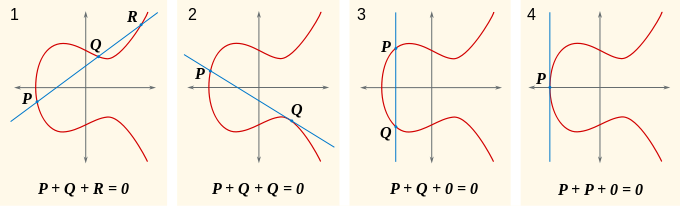
\includegraphics[scale=0.5]{images/EC_group.png}
    \caption{Loi de groupe}
    \label{fig:EC_group}
\end{figure}

\begin{itemize}[label=--]
    \item Lire Implicit differentiation pour le coefficient directeur d'une tangente.
    \item La seule difficulté consiste à prouver l'associativité et ce n'est pas facile. Dans un premier temps, on peut envisager une preuve directe par identification des formules. Mais il faut tenir compte des différentes exceptions. De plus elle s'avère être pratiquement infaisable à la main. On peut se servir de logiciels de calculs formels. Une preuve possible est de montrer qu'une courbe elliptique est isomorphe au groupe de Picard. \href{http://math.rice.edu/~friedl/papers/AAELLIPTIC.PDF}{Preuve élémentaire}.
    \item L'opposé est gratuit. Soit $P = (x, y)$, alors $-P = (x, -a_1x - a_3 - y)$. $-P = (x, -y)$ sur un corps premier et $-P = (x, x+y)$ sur un corps binaire. Cette propriété permet d'accélérer la ECSM via le recodage du scalaire.
    \item L'addition est indépendante des coefficients de la courbe et le doublement ne dépend que du coefficient $a$. Ainsi les formules restent valables pour les courbes vérifiant $a_2 = a$. Un attaquant peut transmettre un point d'une autre courbe de petit ordre. Si aucun test n'est réalisé, l'utilisateur calculera une ECSM sur une courbe faible sans se rendre compte de rien : \emph{Invalid Curve Attacks}. 
    \item De la même façon, on remarque que les formules en X-only (employées par les algorithmes d'échelle) s'appliquent indifféremment sur une courbe ou sur son twist (que se soit pour les courbes de Montgomery ou pour courbes de Weierstrass). Il convient donc de vérifier que les points reçus appartiennent bien à la courbe et non au twist ou bien sélectionner une courbe dont le twist est sécurisé (twist secure). Remarquez que le test peut-être contourné en injectant une faute (cf l'attaque de Fouque et al.).
    \item Une courbe elliptique sur un corps fini est un groupe abélien fini.
    \item Le théorème de Mordell-Weil prouve que $E(\Q)$ est un groupe abélien de type fini, on a ainsi l'isomorphisme suivant $E(\Q) \simeq \Z^r \oplus F$. L'entier $r$ est appelé le rang de $E(\Q)$. En général, il est difficile à déterminer.
    \item $E(\C)$ est isomorphe à un tore.
\end{itemize}


\subsection{Endomorphisme}
On s'intéresse ici aux fonctions définies sur l'ensemble des points d'une courbe elliptique et qui s'expriment comme une fraction rationnelle des coordonnées. Pour cela, il nous faut identifier une écriture rationnelle d'une expression (en $x, y$) faisant intervenir les coordonnées des points de la courbe et donner une signification à l'évaluation de cette écriture aux points de la courbe.

Deux difficultés se présentent :
\begin{itemize}[label=--]
    \item On ne s'intéresse qu'aux valeurs prises par notre fonction rationnelle sur une courbe elliptique. Ainsi ajouter des multiples de l'équation de Weierstrass permet d'obtenir une nouvelle expression qui prendra les mêmes valeurs en tout point de la courbe. Il convient donc d'identifier ces écritures équivalentes.
    \item Il convient ensuite de traiter le cas des dénominateurs nuls et de résoudre le problème de la valeur prise au point à l'infini. L'espace projectif nous sera utile ici.
\end{itemize}

Soit $E_1$ et $E_2$ deux courbes elliptiques affines définies sur \field{}. 
\begin{enumerate}
    \item L'\emph{anneau de coordonnées} $\field{}[E] = \field{}[x,y]/(f(x,y))$. Les éléments de \closure{}$[E]$ sont appelés des polynômes de $E$. Cet ensemble quotient permet d'identifier des écritures équivalentes.
        \begin{itemize}[label=--]
            \item On définit la  \emph{forme réduite} d'un polynôme sur E : $g(x, y) = p(x) + yq(x)$. Le conjugué et la norme : $n(g) = g \hat{g}$.
            \item $n(g)(x_0) = 0 \equiv g(x_0, y_0) = 0$. L'abscisse des zéros d'un polynôme sur $E$ est une racine de sa norme. Ainsi le nombre de zéros d'un polynôme sur $E$ est fini. 
        \end{itemize}
    \item Le \emph{corps des fonctions} $\field{}(E)$ est le corps des fractions de $\field{}[E]$ ou de manière équivalente le corps des fonctions de $E$. Ses éléments sont appelés des \emph{fonctions rationnelles}. On a bien entendu $\field{}[E] \subset \field{}(E)$.
    \item Les fonctions rationnelles ne sont rien d'autres que des fractions rationnelles de \field{}, obéissant à la réduction $f(x, y) = 0$ et que l'on cherche à évaluer en des points de la courbe $E$. Pour cela, il faudrait définir à ces expressions une signification d'application $E \to \mathcal{P}$ : point régulier, pôle, évaluation en \infini{}, ordre d'un point en une fonction : nulle si fini, positive si zéro, négative si pôle, ordre en \infini{}, uniformisante pour déterminer l'ordre d'un point.
    \item Une fonction rationnelle a un nombre fini de zéros et de pôles. \'A une constante près, elle est entièrement déterminée par l'ensemble de ses zéros, de ses pôles et de leurs ordres de multiplicité.
    \item Une \emph{application rationnelle} de $E_1$ dans $E_2$ est une application de la forme $\phi \colon E_1 \to E_2, \phi = [g, h]$ où $g, h \in \field{}(E_1)$ et possédant la propriété que pour tout point $P \in E_1$ où $g$ et $h$ sont définis $\phi(P) = (g(P), h(P)) \in E_2$.\\
    Une application rationnelle définie en chaque point est appelé morphisme. On confond parfois les deux définitions.
    \item Une \emph{isogénie} est un morphisme satisfaisant $\phi(\infini{}) = \infini{}$. Cette propriété est suffisante pour en faire un morphisme de groupes.
    \item Soit $\varphi \colon E_1 \to E_2$ une isogénie. Alors pour tout entier $n$, on a $[n]_{E_1}\varphi = \varphi [n]_{E_2}$. Le kernel d'une isogénie est finie. De plus si \field{} est algébriquement clos, alors $\varphi$ est surjective.
    \item Deux courbes elliptiques sur \GF{q} sont isogènes sur \GF{q} si et seulement si elles ont le même nombre de points \GF{q}-rationnels (et donc le même cardinal quelque soit le corps de base considéré).
    \item Comme $\varphi$ est surjective. Elle induit l'injection suivante sur les corps de fraction associés à $E_1$ et $E_2$ :
    \begin{equation}
        \fonction{\hat{\phi}}{\field{}(E_2)}{\field{}(E_1)}{f}{f\circ \varphi}
    \end{equation}
    L'application $\varphi$ est dite séparable ou inséparable en fonction de la nature de l'extension $\varphi(\field{}(E_2)) : \field{}(E_1)$. Le degré de $\varphi$ correspond au degré de l'extension.
    \item Soit $\phi$ une isogénie de $E_1$ dans $E_2$, où $E_1$ et $E_2$ sont des courbes elliptiques définies sur un corps algébriquement clos. Alors le cardinal de toute fibre (en particulier le noyau) est fini et égal au degré de l'isogénie.
    \item Un \emph{endomorphisme} est une isogénie tel quel $E_1 = E_2$.
    \item $(End(E), +, \circ)$, l'ensemble des endomorphismes de courbes elliptiques est un anneau \footnote{C'est donc une \Z-algèbre. On peut évaluer un polynôme à coefficient entier en un endomorphisme.}. $[m] \in End(E)$, ainsi $End(E)$ contient un sous-anneau isomorphe à \Z. En général ce sont les seuls $\Z \simeq End(E)$, dans le cas contraire (ie : il existe des endomorphismes différent de la multiplication scalaire) on dit que $E$ est à \emph{multiplication complexe}. Les courbes elliptiques sur corps fini sont à multiplication complexe.
\end{enumerate}
Citons trois exemples d'applications rationnelles : les translations, la multiplication scalaire (noté $[m]$) et l'endomorphisme de Frobenius (noté $\phi_q$). Les deux dernières sont des isogénies.
$$\fonction{\phi_q}{E_1(\closure[\GF{q}])}{E_1(\closure[\GF{q}])}{(x, y)}{(x^q, y^q)}$$

Le Frobenius $\phi_q$ est un endomorphisme. Il est important de noter que ce dernier est facilement calculable. En particulier lorsqu'une base normale est utilisée, élevé à la puissance $q$ correspond à un décalage circulaire vers la droite. De plus, pour tout $P \in E(\closure[\GF{q}])$, on a $\phi_q(P) = P$ ssi $P \in E(\GF{q})$. $\phi_q$ vaut l'identité sur $E(\GF{q})$.

Considérons un endomorphisme $\alpha$ :
$$\fonction{\alpha}{E(\closure{})}{E(\closure{})}{(x, y)}{(g(x,y), h(x,y))}$$
En utilisant le fait que $\alpha(-P) = -\alpha(P)$. On peut préciser la forme de $\alpha$ :
$$\alpha(x, y) = (r(x) = p(x)/q(x); y s(x)/t(x))$$
Si $q(x) = 0$, alors $\alpha(x, y) = \infini{}$. Si $q(x) \neq 0$, alors $t(x) \neq 0$.

\begin{definition}
On dit que $\alpha$ est \emph{séparable} si la dérivée de $r(x)$ est non nulle ou si de manière équivalente si la dérivée de $p(x)$ ou $q(x)$ est non nulle. Le \emph{degré} d'un morphisme est le degré maximal entre $p(x)$ et $q(x)$. $deg(\alpha) = max\{deg(p), deg(q)\}$.
\end{definition}

Le théorème suivant est fondamental, il permet de relier le degré d'un endomorphisme au cardinal de son kernel.
\begin{theoreme}
Soit $\alpha \neq 0$ un endomorphisme. Si $\alpha$ est séparable, alors $\# ker\ \alpha = deg(\alpha)$. Sinon $\# ker\ \alpha < deg(\alpha)$.
\end{theoreme}
Dans un morphisme de groupe, toutes les fibres (non vides) ont le même cardinal. Le noyau constitue le cardinal de référence d'une fibre. Le degré d'une isogénie peut s'interpréter comme une borne supérieure du cardinal des fibres du morphisme.

\begin{itemize}[label=--]
    \item $\phi_q$ est non séparable de degré $q$.
    \item La multiplication scalaire par $m$ tel que $pgcd(m, p) = 1$, est séparable et de degré $m^2$.
\end{itemize}

\subsection{Points de torsion}
Soit $m \in \Z$, on considère l'endomorphisme de \emph{multiplication scalaire} suivant : 
$$\fonction{[m]}{E(\closure{})}{E(\closure{})}{P}{[m]P}$$

\begin{definition}
On appelle points de $m$-torsion, les points d'ordre un diviseur $m$.
\begin{equation}
E[m] = ker([m]) = \{ P \in E(\closure{}) \mid mP = \infini{}\}
\end{equation}
Il faut bien remarquer que les points de torsion sont des points \closure{}-rationnels.

\begin{equation*}
E(\field{})[m] \subseteq E[m] \subseteq E(\closure{})
\end{equation*}
L'inclusion s'interprète en tant que sous-groupe.
\end{definition}

\noindent Quelle est la structure des points de torsions ? 

On montre dans un premier temps que la multiplication scalaire est un endomorphisme séparable de degré $n^2$. Pour cela on définit les polynômes de division qui permettent d'expliciter la multiplication scalaire. Puis on utilise le théorème des facteurs invariants ou plus précisément le théorème de structures des groupes abéliens \footnote{Parfois appelé théorème de Kronecker.} et que la multiplication par $N$ s'annule pour conclure. On aboutit au résultat suivant :
\begin{propriete}
Soit $E/\field{}$ une courbe elliptique. Soit $m$ un entier non nul. 
\begin{enumerate}
    \item Si la caractéristique de \field{} est nulle ou si elle ne divise pas $m$, alors 
    $$E[m] \simeq \Zn{m} \times \Zn{m}$$
    \item Si la caractéristique $p$ divise $n$, alors on peut écrire $n = p^r n^{'}$ avec $p\nmid n^{'}$ et on a 
    $$E[m] \simeq \Zn{n^{'}} \times \Zn{n^{'}} \text{ ou } \Zn{p^{r}} \times \Zn{n^{'}}$$
\end{enumerate}
\end{propriete}

Dans le premier cas, les points de $m$-torsions forment un \Zn{n}-module libre de rang 2. On peut donc trouver deux points $S$ et $T$ de $m$-torsion tel que tout point $P \in E[m]$ peut s'écrire de manière unique $P = aS + bT$ avec $a, b \in \left ( \Zn{n} \right )^2$. $(S, T)$ est une base de $E[m]$.

On peut remarquer que le groupe de $n$-torsion est stable par toute isogénie. Ainsi la restriction au groupe de $n$-torsion à toute isogénie peut être représentée par une matrice de taille $2$ à coefficient dans \Zn{}. Soit $\alpha$ une isogénie, nous noterons $\alpha_n$, l'isogénie $\alpha_n$ restreinte à $E[n]$.

\begin{definition}\label{supersingular}
Soit $E$ une courbe elliptique définie sur \GF{q}. On dit qu'elle est \emph{supersingulière} si elle n'a aucun point de $p$-torsion dans \closure[\GF{q}]. Sinon on dit qu'elle est \emph{ordinaire}.
\end{definition}
Une courbe ordinaire possède donc des points d'ordre $char(\field{})$, mais ces points ne sont pas forcément des points \field{}-rationnels.


\section{Courbe elliptique sur un corps fini}
\subsection{Nombre de points}
Une courbe elliptique sur un corps fini est un groupe abélien fini. Tout élément $x \in \GF{q}$ possède au plus deux résidus quadratique. Ainsi le nombre de points est borné par $2q + 1$. (point à l'infini). Peut-on faire mieux ? Commençons par préciser la structure des points \GF{q}-rationnels.

Lorsque $q$ est grand, on a $\# E(\GF{q}) \simeq q$. Cependant pour des applications cryptographiques, il est nécessaire de connaître le nombre exact de points (en particulier le plus grand nombre premier divisant $q$).

\begin{theoreme}(Cassel). 
Soit $E$ une courbe elliptique sur \GF{q}. Alors 
$$E(\GF{q}) \simeq \Zn{n} \hspace{0.5cm} \text{ ou } \hspace{0.5cm} \Zn{n_1} \times \Zn{n_2}$$
pour des entiers $n, n_1, n_2 \geq 1$ avec $n_1 | n_2$ et $n_1 | q-1$.
\end{theoreme}
\begin{preuve}
Théorème de structures des groupes abéliens fini. Possède $n_{1}^k$ points de $n_1$ torsions. On sait qu'il en existe au plus $n_{1}^2$. Ainsi $k \leq 2$.
$E[n_1] \subseteq E(\GF{q}) \implies \mu_{n_1} \subseteq \GF{q}^{*}$
\end{preuve}
Ce théorème montre que les groupes de points d'une courbe elliptique utilisés en cryptographie sont presque toujours cycliques. Une condition nécessaire pour ne pas être cyclique est qu'il existe un nombre premier $p$ tel que $p^2$ divise le cofacteur.

\begin{theoreme}
Théorème de Hasse. L'ordre de $E(\GF{q})$ satisfait 
$$\abs{q + 1 - \# E(\GF{q})} \leq 2\sqrt{q}$$
ou bien $t = q + 1 - \# E(\GF{q})$ avec $\abs{t} \leq 2 \sqrt{q}$. L'entier $t$ est appelé \emph{trace de Frobenius}. Cet entier dépend du corps dans lequel on travail. L'inégalité précédente est appelée \emph{borne de Hasse}.
\end{theoreme}

Une démonstration peut se faire à partir des lemmes suivants :
\begin{itemize}[label=$\bullet$]
    \item $\phi_q (x, y) \in E(\closure[\GF{q}])$.
    \item Un point $(x, y) \in E(\closure[\GF{q}])$ appartient à $E(\GF{q})$ si et seulement si $\phi_q (x, y) = (x, y)$. L'endomorphisme de Frobenius vaut l'identité sur $E(\GF{q})$.
    \item $ker(\phi_q^r - 1) = E(\GF{q^r}), \forall r \geq 1$.
    \item $deg(\phi_q) = q$
    \item L'application $\phi_q^r - 1$ est séparable et donc $\# ker(\phi_q^r - 1) = deg(\phi_q^r - 1)$
    \item L'application degré $d \colon End(E) \to \Z$ est une forme quadratique définie positive.
\end{itemize}

\todo{Théorème de Deuring : pour tout entier $n$ pris dans l'intervalle de Hasse, il existe une courbe elliptique de cardinal égale à cet $n$, à revoir}

\begin{definition}
Le polynôme $X^2 - tX + q$ est appelé polynôme caractéristique de Frobenius (ou polynôme de Weil). L'entier $t$ est appelé la trace de Frobenius.
\end{definition}

\begin{theoreme}
Le polynôme caractéristique de Frobenius est un polynôme annulateur de l'endomorphisme de Frobenius. De plus 
$$Trace((\phi_q)_m) \equiv t \pmod m, \hspace{0.5cm} det((\phi_q)_m) \equiv q \pmod m$$
pour $m$ premier à $p$.
\end{theoreme}
Le polynôme caractéristique de Frobenius est à coefficient entier et $(End(E), +, \circ)$ est un anneau, on peut donc l'évaluer en $\phi_q$. Il est clair que la propriété est vérifiée lorsque $P \in E(\GF{q})$, mais lorsque $P \in E(\closure[\GF{q}])$.

\begin{theoreme}(Weil).
Soit $\# E(\GF{q}) = q + 1 - t$. \'Ecrivons $X^2 - tX + q = (X - \alpha)(X - \beta)$. Alors
\begin{equation}
\# E(\GF{q^n}) = q^n + 1 - (\alpha^n + \beta^n)
\end{equation}
La preuve consiste tout d'abord à montrer $\alpha^n + \beta^n$ est un entier en remarquant que c'est un entier algébrique rationnel. Puis en remarquant que $X^{2n} - (\alpha^n + \beta^n)X + q^n$ est un polynôme annulateur de $\phi_q$. 
\end{theoreme} 

\begin{itemize}[label=$\bullet$]
    \item D'après le théorème de Hasse, l'ordre du groupe $E(\GF{q})$ se trouve dans intervalle de longueur $4\sqrt{q} + 1$. Si on réussit à déterminer un point dont l'ordre est supérieur à cette longueur, alors on retrouve exactement l'ordre du groupe. Même si l'ordre du point est inférieur, on peut restreindre le nombre de possibilités.
    \item Le nombre de points d'une courbe elliptique sur un corps de caractéristique différente de $2$ et $3$ peut se ramener au résidu quadratique. On a $y^2 = f(x)$. Pour chaque $x \in \GF{q}$, on teste si $f(x)$ est un résidu quadratique. Si c'est le cas, alors il existe deux points ayant pour abscisses $x$. Symbole de Legendre.
\end{itemize}

\subsection{Courbes supersingulières}
\begin{definition}
Une courbe définie sur \GF{q} est dite \emph{supersingulière} si elle vérifie l'une des conditions équivalentes suivantes : 
\begin{itemize}[label=--]
    \item $E$ ne possède aucun point d'ordre $p$ dans $E(\closure[\GF{q}])$ (ie : $E[p] \simeq \{ \infini{} \}$)
    \item $\# E(\GF{q}) \equiv 1 \pmod p \Longleftrightarrow a \equiv 0 \pmod p$
    \item $End(E)$ est non commutatif
\end{itemize}
\end{definition}
\begin{proof}
Basé sur deux fais. $s_{n+1} = as_n -qs_{n-1} = \alpha^n + \beta^n$, où $X^2 - aX + q = (X - \alpha)(X - \beta)$. Et le théorème de weil : $\# E(\GF{q^n}) = q^n + 1 - (\alpha^n + \beta^n)$. 
\end{proof}


\begin{propriete}
Soit $E$ une courbe elliptique définie un corps fini \GF{q} de caractéristique $p$. Alors $E$ est supersingulière si et seulement si $p = 2$ ou $3$ et $j(E) = 0$ ou si $p \geq 5$ et $\# E(\GF{p}) = p + 1$ (la trace est nul).
Cette propriété est une conséquence du théorème de Hasse.
\end{propriete}

\begin{itemize}[label=--]
    \item La supersingularité et la singularité sont deux notions distinctes \footnote{Une courbe elliptique est toujours non singulière}. La supersingularité est indépendante du corps de base, elle est liée à l'équation de Weierstrass.
    \item Si $E$ est définie sur un corps binaire, alors la supersingularité de $E$ dépend de la parité de la trace de Frobenius. De manière équivalente de la parité de l'ordre du groupe.
\end{itemize}

\todo{Mettre lemme : $E[l] \subseteq E(\GF{q^k}) \implies \mu_l \subseteq \GF{q^k}^{*}$}

\begin{definition}
Soit $E$ une courbe elliptique définie sur \GF{q}. Soit $l$ l'ordre d'un point \GF{q}-rationnel de $E$. On appelle \emph{degré de plongement} de $l$ (par rapport à $E(\GF{q})$), le plus petit entier naturel non nul $k$ tel que $l | (q^k -1)$. Autrement dit le degré de plongement est le degré de la plus petite extension de \GF{q} contenant $\mu_l$.
Par abus de langage, quand on parle de degré de plongement de $l$, on sous-entend qu'il existe un point \GF{q}-rationnel d'ordre $l$.
\end{definition}

\todo{Mettre théorème de Balasubramanian - Koblitz}

\begin{theoreme}
Le degré de plongement d'une courbe supersingulière est inférieur ou égal à $6$. Plus précisément :
\begin{itemize}[label=$\bullet$]
    \item en caractéristique $2$, on a $k \leq 4$
    \item en caractéristique $3$, on a $k \leq 6$
    \item lorsque $p \geq 5$, on a $k \leq 2$
\end{itemize}
De plus les bornes sont atteintes.
\end{theoreme}

L'utilisation de courbes supersingulières en cryptographie est attrayante. En effet on peut envisager de coder le scalaire en base $q$ et de calculer les $[q^i]P_j$ à l'aide du Frobenius\footnote{Il faut néanmoins considérer une extension du corps de base.}. La trace de cette famille de courbes étant nulle, le calcul précédent s'en trouve simplifié. En 1990, Menezes et Vanstone avaient proposé d'employer cette technique sur des courbes binaires supersingulières.
Malheureusement les courbes supersingulières sont faibles : leur degré de plongement est petit. Cette particularité rend praticable l'attaque MOV qui transfert un log discret d'une courbe vers un log discret sur un corps fini\footnote{C'est une extension du corps de base de degré égal au degré de plongement.}. Toutefois cette famille de courbes est intéressantes dans le cadre des couplages.



\section{Couplage}
\subsection{Définition}
Les couplages sont une notion mathématique apparut en cryptographie dans les années 90. Les premiers introduit en cryptographie sont les couplages de Weil et de Tate. Dans un premier temps, les couplages ont été utilisés dans un but destructeur. En effet ces applications permettent de transférer le logarithme discret d'une courbe elliptique en un logarithme discret sur un corps fini (où se problème est plus facile à résoudre \footnote{\'{A} condition que le corps fini ne soit pas trop grand.}). La première attaque de ce type est l'attaque MOV \footnote{Du nom de ses auteurs : Menezes, Okamoto et Vanstone} en 1993 basée sur le couplage de Weil. L'attaque Frey Rück 1994 est quant à elle basée sur le couplage de Tate. 

Les couplages ont ensuite permis la construction de protocoles originaux : échange de clé tri-partite en un tour par A. Joux en 2000, cryptographie basé sur l'identité, schémas de signatures courtes.

\begin{definition}
Soient $G_1, G_2$ deux groupes d'exposant $n$ notés additivement et $G_3$ un groupe cyclique d'ordre $n$ noté multiplicativement. Un couplage est une application : 
$$e \colon G_1 \times G_2 \to G_3$$
qui est 
\begin{itemize}[label=--]
    \item bilinéaire : pour tout $P \in G_1, Q \in G_2, a \in \Zn{n}$, on a $e([a]P, Q) = e(P, Q)^{a} = e(Q, [a]Q)$
    \item non dégénérée : pour tout $P \in G_1 \ \{ 0 \}$, il existe $Q \in G_2$ tel que $e(P, Q) \neq 1$; de même pour tout $Q \in G_2 \ \{ 0 \}$, il existe $P \in G_1$ tel que $e(P, Q) \neq 1$. Se simplifie lorsque $G_1$ = $G_2$ est un groupe cyclique. 
    \item Facilement calculable.
\end{itemize}
\end{definition}


\subsection{Couplage de Weil}
\begin{theoreme}
Soit $E$ une courbe elliptique sur un corps parfait \field{}. Soit $n$ un entier premier avec la caractéristique de \field{}. Alors $E[n] \simeq (\Zn{n})^2$, $\mu_n$ est le groupe des racines $n^{ieme}$ de l'unité, cyclique.
Il existe un couplage $e_n \colon E[n] \times E[n] \to \mu_n$ appelé \emph{couplage de Weil} vérifiant les propriétés suivantes :
\begin{itemize}[label=--]
    \item Bilinéaire.
    \item Antisymétrique. $\forall S, T \in E[n], e_n(S, T) = e_n(T, S)^{-1}$
    \item Identité (ou alterné). $\forall T \in E[n], e_n(T, T) = 1$.
    \item Non dégénérée. Si $e_n(S, T) = 1$ pour tout $T \in E[n]$, alors $S = \infini{}$ et inversement.
    \item Galois-invariant. $e_n(\sigma S, \sigma T) = \sigma (e_n(S, T))$ pour tout \field{}-automorphisme $\sigma \in Gal(\closure{}/\field{})$.
    \item Endomorphisme de $E$. $e_n(u(s), u(T)) = e_n(S, T)^{deg(u)}$ pour tout endomorphisme $u \in End_{\closure{}}(E)$.
\end{itemize}
\end{theoreme}

\todo{Voir lien entre les deux defs de non dégénéré. L'identité est-elle une conséquence de l'antisymétrie ?}

\begin{corollaire}
Dans les mêmes conditions que précédemment, $E[n]$ est un \Zn{n}-module libre de rang $2$. Soit $\{T_1, T_2\}$ une \Zn{n}-base, alors $e_n(T_1, T_2)$ est une racine primitive n-ième de l'unité.
\end{corollaire}

\begin{corollaire}
Si $E[n] \subseteq E(\field{})$, alors $\mu_n \subseteq \field{}$.
\end{corollaire}

L'invariance de Galois montre que si $P_1$ et $P_2$ sont définis sur une extension \GF{q^d}, alors le couplage $e_n(P_1, P_2)$ appartient à \GF{q^d}. L'algorithme de Miller permet alors de calculer ce couplage de façon effective avec une complexité en $O(log(n))$ opérations dans $E(\GF{q^d})$.


\subsection{Applications}
\begin{itemize}[label=--]
    \item Résous le problème de Diffie Helman Décisionnel. Connaissant $[a]P, [b]P, [c]P$ et $P$, déterminer si $[c]P = [ab]P$. La difficulté est que l'on ne conait pas $[ab]P$ mais avec un couplage on a $e([a]P, [b]P) = e(P, [ab]P)$.
    \item Transfert du logarithme discret. Si $Q = [k]P$, alors on a $e(T, Q) = e(T, P)^k$. Ainsi $k = log_{P}(Q) = log_{e(T,P)}(e(T, Q))$. On transfert ainsi un log discret d'une courbe elliptique sur un corps fini. On peut procéder de la même façon si on possède un morphisme des points rationnels d'une courbe à valeurs dans un corps fini.
    \item \'{E}change de clé tripartite due à A. Joux en 2000. Chaque entité génère un couple de clé éphémère et diffuse aux deux autres participant sa clé publique. Le secret partagé correspond à $e([b]P, [c]P)^a = e(P, [abc]P)$. La nouveauté du protocole de Joux est que trois participant peuvent s'échanger un secret en un seul tour. En effet les messages échangés sont indépendant les uns des autres. Les mêmes problèmes d'authenticité que pour le DH naïf apparaissent : authentification des messages via une signature et authentification des clés publiques via un certificat issue d'une autorité de confiance.
    \item Cryptographie basée sur l'identité : introduit par Shamir en 1984. La cryptographie à clé publique traditionnelle nécessite la mise en place d'une infrastructure à clé publique (PKI) afin de garantir l'authenticité des clés publiques. Cela se fait via la mise en  \oe{}uvre d'une autorité de certification. Les schémas basés sur l'identité \footnote{Identity Based Encryption} permettent de se passer des certificats électroniques, réputés pour leur complexité. Les clés publiques sont les identités des entités. Les clés privées sont construites par le PKG \footnote{Private Key Generator}, aussi appelé autorité de confiance, et transmises aux utilisateurs.
    
    Par leur construction, les schémas basés sur l'identité (IBE) parviennent à résoudre les problèmes liés à l'authentification, à la gestion et à la révocation des clés publiques, néanmoins ils nécessitent la présence d'une autorité ultra-puissante (Private Key Generator) qui fournit à chaque utilisateur la clé privée correspondante à sa clé publique. La confiance accordée à cette autorité doit être sans faille, car elle est intrinsèquement capable de régénérer la clé privée de tout utilisateur, et par conséquent capable de réaliser sans autorisation des signatures ou des déchirements.
    
    La toute puissance de la PKG n'est pas forcément une mauvaise chose. Cette particularité peut même s'avérer intéressante dans une entreprise ou à des fins militaires. Cependant la non-répudiation des signatures n'est maintenant plus assurée. La législation européenne impose que les clés privées de signatures soient sous le seul contrôle de leurs propriétaires.
    
    Alice veut envoyer un message chiffré à Bob.
    \begin{enumerate}
        \item Alice chiffre son message en utilisant : l'identité de Bob (son adresse mail par exemple) et la clé publique du PKG.
        \item Bob obtient sa clé privée auprès du PKG après s'être authentifié. Sa clé privée dépend de son identité et de la clé privée du PKG appelée clé maître.
    \end{enumerate}
    Premier protocole fournit par Boneh et Franklin en 2001. \href{http://www.azhari-crypto.org/wp-content/uploads/Accouplements_et_cryptographie_bas%C3%A9e_sur_lidentit%C3%A9.pdf}{Lien}. Des chercheurs japonais avait proposé en mai 2000 un schéma de chiffrement basé sur l'identité basé sur les couplages. Mais leur article avait été publié en japonais.                                                                                                                                                                                                                                 
    \item Signatures courtes : schéma de signatures courtes BLS \footnote{Boneh-Lynn-Shacham.} en 2001.
\end{itemize}

\chapter{Cryptographie sur les courbes elliptiques}
Une courbe elliptique est une courbe plane régit par une équation de forme particulière, dont les points possèdent la propriété remarquable de pouvoir être additionnés entre eux. On peut donc, étant donné un point $P$ et un entier $n$, définir le point $Q = nP$ comme $Q = P + P + \ldots + P$ (où $P$ apparaît $n$ fois). En cryptographie, on utilise des points à coordonnées discrètes de grandes tailles (typiquement un corps premier ou aussi une extension d'un corps binaire, de 200 bits). $P$ étant donné, $Q$ peut être rapidement calculé par ordinateur même lorsque $n$ est lui aussi de grande taille. L'inverse est faux : de façon surprenante on ne connaît aucune méthode efficace de retrouver $n$ à partir de $P$ et $Q$. Ce problème difficile, appelé \emph{problème du logarithme discret sur courbe elliptique} \footnote{On trouve aussi parfois le terme logarithme elliptique.}, permet de concevoir des algorithmes à clé publique en choisissant $n$ comme clé secrète et $Q$ comme clé publique.

Introduite dés 1985, l'ECC \footnote{Elliptic Curve Cryptography : Cryptographie sur Courbes Elliptiques} se déploie progressivement. On la retrouve aussi bien dans le monde Internet/Web (TLS, SSH, Bitcoin) que dans la télévision à péage (Viaccess), la téléphonie (SIM) ou l'identification (passeports).

\todo{Expliqué rapidement l'utilisation des courbes elliptiques en crypto. Expliquer qu'il existe différentes familles de courbes qui possèdent chacunes leurs spécificités : formule unifiée, différents système de coordonnées, choix de l'algorithme de multiplication scalaire régulier ou non, utilisation d'endomorphisme, choix de représentation des éléments \ldots}

\section{Vue générale}
L'utilisation des courbes elliptiques en cryptographie a été proposée en 1985 indépendamment par Victor Miller et Neal Koblitz. L'ensemble des points d'une courbe elliptique peut être munie d'une structure de groupe (d'une addition). L'addition de points d'une courbe elliptique à coordonnées réelles s'interprètent facilement de manière géométrique. L'idée consiste d'utiliser le groupe des points d'une courbe au problème de logarithme discret. La principale raison de son attrait est qu'on ne connaît aucun algorithme sous-exponentiel résolvant le problème du logarithme discret sur des courbes elliptiques bien choisies. Ce qui conduit à des tailles de paramètres significativement plus petit que les cryptosystèmes tel que RSA ou DSA pour un même niveau de sécurité. Ainsi plus le niveau de sécurité est grand et plus ce fossé est important. Des tailles de clé plus faibles permettent des calculs plus rapides, une réduction de l'espace de stockage, de bande passante et de puissance de traitement \footnote{Bandwith, processing power.}.

L'utilisation des courbes elliptiques nécessite d'effectuer un certain nombre de choix : choix du cryptosystème, du modèle de la courbe et de ses coefficients, du corps fini, de l'algorithme de multiplication scalaire, des algorithmes pour les opérations dans le corps de base \ldots Chacune de ces applications peuvent avoir un impact significatif sur la performance globale de notre application.

Avant de pouvoir décrire une méthode, un procédé de génération de courbes elliptiques, il faut au préalable recenser l'ensemble des attaques connues. Chacune de ces attaques met en lumière une faille potentielle dans l'utilisation des ECC. Elles signalent que tel ou tel choix de courbes, de paramètres doivent être éviter, que ces derniers doivent vérifier une certaines propriétés. On obtient une condition nécessaire pour atteindre un niveau de sécurité. La condition suffisante se fait via la notion de réduction.

La cryptographie sur courbes elliptiques se décompose en plusieurs couches. Choix du protocole, algorithme de multiplication scalaire, formules d'addition et de doublement et enfin opérations dans le corps de base. 

\begin{figure}[ht]
    \centering
    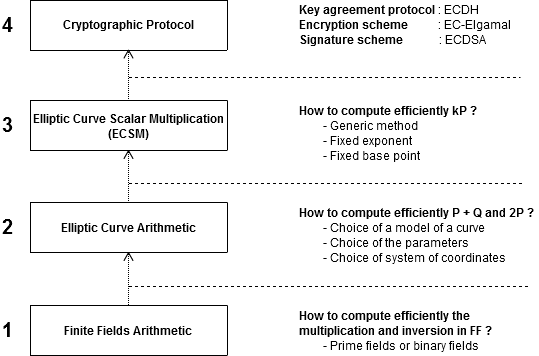
\includegraphics[scale=0.7]{images/ECC_level.png}
    \caption{Hiérarchie, couches dans l'utilisation des courbes elliptiques en cryptographie}
    \label{fig:my_label}
\end{figure}
\FloatBarrier

\section{Intérêt des courbes elliptiques en cryptographie}
Nous résumons ici les attraits (et points faibles) de la cryptographie sur courbe elliptique par rapport à la cryptographie asymétrique classique.
\begin{itemize}[label=$\bullet$]
    \item Excepté pour quelques familles courbes, il n'y pas de meilleurs attaques connues que les attaques génériques pour résoudre le problème du logarithme discret.
    \item Le corps de base est plus petit que celui de RSA ou du logarithme discret sur un corps finis pour un même niveau de sécurité : $224$ bits au lieu de $2048$ pour $128$ bits de sécurité. Actuellement le gain est de l'ordre d'un facteur $10$.
    \begin{itemize}[label=--]
        \item Arithmétique du corps de base plus facile à implémenter et plus efficace.
        \item Clés plus petites qu'avec RSA (sauf pour la clé publique), actuellement différence de l'ordre d'un facteur $10$.
        \item Génération de clé facile (contrairement à RSA).
        \item ECC plus rapide que le DL sur corps finis.
        \item ECC plus rapide que RSA pour les opérations privées mais pas pour les opérations publiques si on choisit $e = 3$. La vérification des signatures est donc un peu plus efficace.
    \end{itemize}
    \item Ce fossé entre ECC et les autres systèmes s'accroît (attaques exponentielles contre sous-exponentielle). Plus le temps passe, plus la puissance des ordinateurs est grande. Augmenter le niveau de sécurité requiert d'augmenter davantage la taille de clés de RSA que de ECC.
    \item Création de protocoles originaux en utilisant les couplages : échange de clé tri-partite, chiffrement basé sur l'identité, signatures courtes.
\end{itemize}

ECC versus RSA : \cite{koblitz2011elliptic}. Au départ l'arrivée des courbes elliptiques en cryptographie a suscité parmi les cryptographes la curiosité et l'approbation. Bien que la plupart des chercheurs n'avait jamais étudié les courbes elliptiques et n'en avait qu'une compréhension limitée, ils avaient tendance à réagir positivement. 
Puis création de la compagnie Certicom : ECC devient alors une menace commerciale à le RSA. 


{\renewcommand{\arraystretch}{1.3}
\begin{table}[h]
\centering
    \begin{tabular}{|c||c|c|c|c|c|}
        \hline
        Niveau de Sécurité en bits & $80$ & $112$ & $128$ & $192$ & $256$\\
        \hline
        Module RSA en bits & 1024 & 2048 & 3072 & 8192 & 15360 \\
        \hline
        ECC : Taille du corps de base en bits & $160$ & $224$ & $256$ & $384$ & $521$ \\
        \hline
    \end{tabular}
\caption{Comparatifs des tailles des clés pour différents niveau de sécurité entre RSA et ECC}
\label{tab:keylength}
\end{table}}
Le site \href{http://www.keylength.com}{KeyLength} liste les recommandations d'agences gouvernementales concernant la taille minimale des clés a adopté. La plupart préconise $112$ bits de sécurité environ.

\begin{comment}
\begin{figure}[scale=0.4]
\centering
    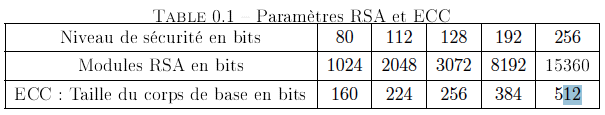
\includegraphics[scale=0.5]{images/paramRSAECC.png}
    \caption{Comparatifs des tailles des clés pour différents niveau de sécurité entre RSA et ECC}
    \label{fig:keylength}
\end{figure}
\end{comment}

\section{Standards et brevets}
Au cours des années 2000, différentes courbes ont été standardisées. Certaines sont d'ailleurs données sans aucunes justifications. 
\begin{description}
    \item[NIST\footnote{NIST : National Institute of Standards and Technologie.}] \hfill \\ Spécification en 1999 de $15$ courbes : $5$ sur corps premiers, $5$ sur corps binaire et $5$ courbes de Koblitz. Forme de Weierstrass, nombre de Mersenne Généralisé, $a=-3$ et $b$ pseudo-random, co-facteur minimal ($2$ pour corps binaires et $2$ ou $4$ pour Koblitz).
    \item[SECG\footnote{SECG : Standards for Efficient Cryptography Group.}] \hfill \\
    Provient de la société canadienne Certicom, rachetée par BlackBerry. Date de 2009. Ce standard reprend certaines courbes du NIST (par exemple P-$256$ et secp256r1 correspondent à la même courbe). De plus il possède la particularité de proposer des courbes GLV avec $a = 0$ ou $b = 0$. Le protocole Bitcoin utilise une de ces courbes particulière, la secp256k1, mais sans tirer partie de l'endomorphisme facilement calculable associé.
    \item[Brainpool\footnote{Consortium Européen dirigé par la BSI qui l'analogue de l'ANSSI germanique.}] \hfill \\
    Date de 2005 (puis révisé en 2010). Procédé de génération de courbes plus rigides, du moins en apparence (les décimales de $\pi$ forment la graine pour le choix des nombres premiers et $\exp(1)$, la constante d'Euler, pour les coefficients de la courbe), forme de Weierstrass, $a$ et $p$ pseudo-aléatoire, non twist-secure.
    \item[Organismes Gouvernementaux] \hfill \\
    Données sans aucunes justifications. La Chine en 2010 a proposé OSCCA SM2 et la France par le biais de l'ANSSI en 2011, ANSSIFRP256v1 ou FRP256v1, paru aux JO \href{http://www.legifrance.gouv.fr/affichTexte.do;jsessionid=?cidTexte=JORFTEXT000024668816&dateTexte=&oldAction=rechJO&categorieLien=id}{ici}. Nombre premier pseudo-random et $a=-3$.
    \item[Académiques et Industriels] \hfill
        \begin{itemize}[label=--]
            \item Curve25519\footnote{Conventions : Curve$|d|$ pour les courbes d'Edwards avec le coefficient $d$, la taille du corps de base n'est donc pas spécifiée. Et on a Curve$m\delta$ pour les courbes de Montgomery sur $\GF{2^m - \delta}$. La convention utilisée ne permet pas toujours d'identifier clairement le modèle de courbe choisi.}, Curve41417 proposées par Bernstein et Lange. La première est une courbe de Montgomery définie sur $\GF{2^{255}-19}$ et est birationnellement équivalente à Ed25519.
            \item NUMS\footnote{NUMS : Nothing Up My Sleeve} Curves, proposées par l'équipe de Microsoft et Bos de NXP. \href{http://research.microsoft.com/pubs/219966/curvegen.pdf}{Lien.}
            \item Goldilocks448 ou Ed448-Goldilocks proposée par Hamburg. Appelé ainsi en référence au nombre d'or et à la forme du nombre premier. $p = 2^{448} - 2^{224} -1$.
            \item M-221, M-383, M-511, E-222, E-382, E-521. M pour Montgomery et E pour Edwards. Proposition de six nouvelles courbes à des niveaux sécurités similaires de ceux du NIST, complète les Curves. \href{https://eprint.iacr.org/2013/647.pdf}{Lien.} Ce papier résume les caractéristiques de la Curve25519. Il existe la Ridinghood curve seul change le nombre premier. $p = 2^{480} -2^{240} -1$.
            \item Ted127-glv4, Four$\mathbb{Q}$.
        \end{itemize}
\end{description}

Présentation intéressante, \href{http://www.imsc.res.in/~ecc14/slides/costello.pdf}{lien.} IRTF CFRG préconise l'adoption des courbes Curves25519 et Goldilocks448 pour l'inclusion dans les futures versions de TLS.

\vspace{0.5cm}

L'existence de brevets dans l'univers de la cryptographie sur courbe elliptique est un des facteurs limitant une acceptation plus générale, notamment pour les courbes binaires. Déposés notamment par le sociétés Certicom et Cryptography Research, ils protègent plus souvent des techniques d'implémentation que des courbes et des algorithmes proprement dits. Les brevets ne sont pas un frein très grand au déploiement et à l'adoption des courbes elliptiques en cryptographie. Aux quelques brevets existant, des solutions alternatives existent. 

Rappelons que Certicom \footnote{Racheté par Blackberry en 2009} est une société canadienne fondée par Scott Vanstonne, connu notamment pour l'algorithme DSA\footnote{Digital Signature Algorithm}. Cryptography Research est la société fondée par Paul Kocher. 

\noindent Quelques techniques sujettes aux brevets : 
\begin{itemize}[label=--]
    \item Nombres premiers sous une forme spéciale : Mersenne, pseudo-Mersenne ou Crandall, Mersenne Généralisé.
    \item Bases normales.
    \item Techniques de compression.
    \item Protocole d'échange de clé MQV.
    \item Techniques GLV.
\end{itemize}

Noter que la NSA en 2003 a racheté les droits de certains brevets sur ECC (notamment ceux sur MQV) dans un deal de $25$ millions de dollars et distribuent des licences à des compagnies américaines.

Remarques de Bernstein \footnote{\href{https://cr.yp.to/newelliptic/nistecc-20160106.pdf}{Failures in NIST ECC standards.}} : As far as we know, the most important ECC patents have all expired, and the entire core of ECC is now patent-free. Some fringes of ECC are still patented. The most interesting remaining patents are the GLV patents; these patents cover the use of endomorphisms to speed up ECC on special curves (GLV curves, GLS curves, \Q-curves, and so on).



\section{Dates notables}
\begin{itemize}
\item 85 : Introduction des courbes elliptiques en cryptographie indépendamment par Koblitz et Miller.
\item 87 : Courbes de Montgomery.
\item 89 : Introduction des courbes hyperelliptiques en cryptographie par Koblitz.
\item années 90 : apparition des couplages.
\item 93 : Attaque de Menezes-Okamoto-Vanstone (MOV) puis amélioration par Frey-Rück sur les courbes munient d'un petit degré de plongement.
\item 99 : Attaque de Smart-Semaev-Satoh-Araki sur les courbes anomales.
\item 99 : Spécifications des courbes du NIST.
\item 00 : \'Echange de clé tripartite à un tour d'A. joux.
\item 01 : Première réalisation effective d'un cryptosystème basé sur l'identité (IBE)\footnote{Identity Based Encryption : problème posé par Shamir en 84.} proposé par Boneh et Franklin à Crypto. Le cryptologue britannique Cocks\footnote{Qui a notamment découvert une variante de RSA quelques années plus tôt au sein du GCHQ.}, a proposé la même année un système IBE basé sur la résiduosité quadratique modulo deux nombres premiers.
\item 01 : Gallant, Lambert, Vanstone ont proposé une méthode appelé GLV à Crypto afin d'accélérer la multiplication scalaire à l'aide d'endomorphisme.
\item 06 : Proposition de la courbe Curve25519 (Montgomery) par Bernstein. 
\item 07 : Courbe d'Edwards, et les tordues d'Edwards l'année suivante.
\item 09 : standard de Certicom, nommé SECG v2.
\item 09 : Galbraith, Lin et Scott étendent la méthode GLV en construisant des endomorphismes efficient sur les twists de $E(\GF{p^2}$. La méthode GLS peut être appliquée aux courbes GLV on est ainsi muni de deux endomorphismes efficient permettant une décomposition en dimension 4.
\item 05 et 10 : courbes du Brainpool. Consortium européen dirigé par la BSI (analogue germanique de l'ANSSI).
\item 13 : \Q{}-curves proposées par Smith.
\end{itemize}

\chapter{Problème du Logarithme Discret}
\todo{retrouver ma fiche sur DLP}
Survey de février 2014 d'Antoine Joux sur le DLP \href{https://www1.lip6.fr/~pierrot/papers/DlogSurvey.pdf}{Survey}.

\todo{Introduction du problème (DLP, DDLP, CDLP + EC), définir les notations, algorithme générique (black-box groups), théorème de Shoup, objectif en crypto, recherche exhaustive \ldots}

D'un côté, on a les algorithmes génériques. Le théorème de Shoup fournit une borne inférieure sur la complexité d'un algorithme générique. On connaît des algorithmes optimaux de résolution du problème du logarithme discret dans un cadre générique. 

D'un autre côté, on a les algorithmes non génériques qui vise à tirer partie des spécificités du groupe afin d'obtenir des algorithmes de complexité sous-exponentielles c-à-d meilleurs que les algorithmes génériques. 

Le groupe des points d'une courbe elliptique est optimal pour le DLP. Excepté pour quelques familles de courbes, aucun algorithme non génériques existe.

\section{Algorithmes génériques}

\subsection{Algorithme de Silver-Pohlig-Helman}
\begin{itemize}[label=$\rightarrow$]
    \item Cet algorithme a des répercussions importantes.
    \item En pratique, si l'ordre du point de base est quelconque alors on utilise cet algorithme puis pour chaque sous-problème, une des méthodes suivantes est utilisées. 
\end{itemize}


\subsection{Baby Step Giant Step (BSGS)}
Aussi appelé algorithme de Shanks.

\subsection{Algorithme Rho de Pollard}
Paradoxe des anniversaires : combien doit-on réunir de personnes afin que la probabilité que deux d'entre eux aient la même date d'anniversaire soit supérieur à $1/2$ ? $23$ suffit ! Il ne s'agit pas en réalité d'un paradoxe mais seulement d'un fait contre-intuitif. 

Dans un groupe de $n$ personnes quelle est la probabilité que deux d'entre elles fêtent leur anniversaire le même jour ? On se donne $\mathcal{U}$ un ensemble de cardinal $n$. On effectue $k$ tirages avec remise. Les boules sont tirées de manières uniforme.
\begin{itemize}
    \item Quelle est la probabilité d'obtenir une collision ? ie : calculer $\mathcal{P}(n, k)$, tirer deux fois la même boule. Ou de manière analogue, par complémentarité, quelle est la probabilité que les boules tirées soient toutes distinctes ? ie : que l'on obtienne aucune collision, calculer  $1 - \mathcal{P}(n, k)$. Dans ce cas, $k < n$ sinon cette probabilité est nulle. 
    \item Fixons $n$ la taille de notre urne. On se donne un seuil $\alpha \in [0, 1]$. Combien doit-on effectuer de tirages afin d'obtenir $\mathcal{P}(n, k) \geq \alpha$ ? ie : obtenir une collision avec une probabilité supérieur ou égal à $\alpha$.
    \item Théorème : Si des éléments sont tirés de manière aléatoire d'un ensemble $\mathcal{U}$ alors le nombre de tirage attendu avant d'obtenir une collision est $\sqrt{\pi n / 2}$ où $n = \# U$.
\end{itemize}

Le problème des anniversaires se reformule en terme de collision ce qui aura son importance lors de l'étude des fonctions de hachages.

Si une fonction de hachage a une sortie de $N$ bits, alors 

\href{http://www.lifl.fr/~wegrzyno/portail/PAC/Doc/Cours/paradoxeAnniversaire.pdf}{Lien}


\subsection{Algorithme du kangourou de Pollard}
Pollard’s Kangaroo method is based on running two independent random walks on a cyclic group G, one starting at a known state (the "tame kangaroo") and the other starting at the unknown but nearby value of the discrete logarithm x (the "wild kangaroo"), and terminates after the first intersection of the walks. As such, in order to analyze the algorithm it suffices to develop probabilistic tools for examining the expected time until independent random walks on a cyclic group intersect, in terms of some measure of the initial distance between the walks.

Cette méthode est appelée soit la méthode lambda de Pollard ou la méthode du kangourou apprivoisé et sauvage.


\subsection{Logarithme discret en groupe}
\todo{Mettre la footnote dans le titre.}

\footnote{Batch discrete logarithm.}
Cf. Safecurves et article de générations de courbes à la volée.


\section{Algorithmes non génériques}
\subsection{Calcul d'indice}
\todo{Rappeler le principe général de l'algorithme dans \GF{p}. Donner les derniers résultats dans ce domaine cf Antoine Joux et ses doctorants. Mentionner l'existence d'un algorithme similaire pour les courbes hyperelliptiques de genre supérieur ou égal à 3. Expliquer brièvement pourquoi il n'existe pas d'algorithme similaire aux courbes hyperelliptiques de genre 1 et 2.}


\subsection{Xedni calculus}
Algorithme de Silverman en 98. Le nom Xedni vient de indeX à l'envers. Allez voir \cite{koblitz2011elliptic}.

\todo{Donner seulement les conséquences de cet algorithme, cf article de Koblitz sur l'histoire d'ECC.}

\chapter{Protocoles sur EC}
\todo{\'Ecrire les algorithmes en Latex.}

\noindent On se donne les paramètres suivants : 
\begin{itemize}[label=$\bullet$]
    \item Soit $E$, une courbe elliptique définie sur un corps fini \GF{q}.
    \item Soit $P$, un \GF{q}-point rationnel d'ordre $l$, où $l$ est le plus grand facteur premier du cardinal de la courbe. $P$ est appelé le \emph{point de base} et le sous-groupe principal est le sous-groupe engendré par $P$.
\end{itemize}

Le \emph{cofacteur} $h$ est l'ordre du groupe $\#E(\GF{p})$ divisé par son plus grand facteur premier $l$. On a $\#E(\GF{p}) = hl$. Pour des raisons d'efficacité, on choisit $h$ le plus petit possible. Par exemple NIST préconise des courbes elliptiques avec un cofacteur égal à un.

Une \emph{clé privée} est entier $k$ choisi aléatoirement dans $\{1, \ldots, l-1\}$. La \emph{clé publique} correspondante est le point $P_k = [k]P$.

\section{Protocoles d'échange de clé}
\todo{Résumé : key establishment. Ou faire ce résumé dans crypto et mettre un lien.}
\subsection{ECDH : Ellptic Curve Diffie Hellman}
ECDH est un protocole d'échange de clé publié en 1976 par Diffie et Hellman dans leur célèbre article \og New directions in Cryptography \fg{}. Cependant Ellis, Cocks et Williamson qui travaillaient pour les services de renseignements britanniques (GCHQ) avaient déjà découvert ce procédé quelques années plus tôt. De plus il faut savoir que malgré le nom trompeur du protocole, que Merkle \footnote{Il est aussi à l'origine du procédé de construction de Merkle-Damgard pour les fonctions de hachages.} a aussi participé à cette découverte.
\begin{algorithm}
    \caption{ECDH}
    \label{ECDH}
    \begin{algorithmic}[1]
    
        \REQUIRE
        \ENSURE 
        \STATE $(i, j)$ \hspace{1.04cm} $\leftarrow $  
    \end{algorithmic}
\end{algorithm}

\begin{itemize}[label=$\bullet$]
    \item Rappelons que l'objectif d'un DH est le partage d'un secret (une chaîne de bits quelconques) entre Alice et Bob. Ce secret n'est jamais utilisé tel quel comme clé privée d'un algorithme symétrique. La raison est que la clé privée d'un algo symétrique doit être de longueur fixé et uniformément distribué (d'entropie maximale). Le secret est utilisé comme l'entrée d'une fonction de dérivation de clé KDF \footnote{Key Derivation Function.} qui construit un ensemble de clé appelé \emph{clé de session}. On peut ainsi changer de clé symétrique sans refaire un ECDH.
    
    \item ECDH, bien plus rapide que DH sur un corps fini, se décline en deux versions. 
        \begin{enumerate}
            \item ECDHE : ECDH éphémère. Protocole habituellement présenté. C'est un accord de clé : les deux parties influencent la valeur du secret partagée. De plus il possède la propriété de cryptographie persistante \footnote{Forward Secrecy} : la compromission de la clé privée statique de long terme ne compromet pas la confidentialité des communications passées. En effet cette clé n'est utilisée que pour signée et n'intervient pas dans la construction du secret. 
            \item ECDH statique ou à un pas. C'est un transport de clé : seul un des participant définit le secret. L'avantage est que les deux parties n'ont pas besoin d'être connecté. Cette version assure uniquement une authenticité unilatérale. Cette caractéristique peut s'avérer intéressante. Par exemple pour le protocole SSL \ldots A revoir.
        \end{enumerate}
        
    \item Protocole vulnérable à une attaque active de type man-in-the-middle. Comment s'assurer que le message reçu (clé publique éphémère) provient bien d'Alice ? Pour éviter cette attaque, il est nécessaire que les messages échangés entre Alice et Bob soient authentifiés. Pour cela, Alice doit signer la clé publique éphémère qu'elle envoie avec ECDSA et sa clé publique de long terme. Elle envoie ainsi : $(aG, (r, s))$. On parle dans ce cas de ECDHE-ECDSA.
    
    \item Cela n'est pas toujours suffisant. Il faut aussi s'assurer de l'authenticité de la clé publique. La clé publique me permettant de vérifier la signature est-elle bien celle d'Alice ? Pour cela on a recourt à la notion de certificat (permet de lier l'identité d'une entité à sa clé publique) et d'une autorité de confiance. On transfert le problème d'authenticité de la clé publique d'Alice à l'authenticité de la clé publique d'une autorité de confiance appelée \emph{clé racine}.
    
    \item Lorsque l'on reçoit une clé publique (un point), il faut s'assurer que c'est un point de la courbe et qu'il est d'ordre $l$ ie : qu'il appartient au sous-groupe principal (Procédure de validation de clé). Un attaquant peut envoyer un point de petit ordre et ainsi calculer le log discret de ce point. Il récupère la valeur de la clé secrète modulo l'ordre de son point. Il peut réitérer ce procédé puis utiliser le CRT. Un point qui n'appartient pas à la courbe ne doit jamais être accepté. Si le point appartient à la courbe mais est d'ordre $h$, l'attaquant ne gagnera pas grand chose, on peut utiliser le ECDH-cofacteur. 
    
    \item En pratique, on utilise généralement des techniques de compression de points. Mais on peut faire encore mieux : courbes de Montgomery.
\end{itemize}

\subsection{ECMQV : Menezes-Qu-Vanstone}
MQV est un protocole d'échange de clé authentifié basé sur le schéma de Diffie-Hellman. Il a été initialement proposé par Menezes, Qu et Vanstone en 1995 et modifié par Law et Solinas en 1998. Schéma breveté par Certicom.

\section{Schémas de chiffrement}
\subsection{EC-ElGamal : Elliptic Curve ElGamal}
Elgamal est un Diffie-Hellman déguisé. L'algorithme de chiffrement consiste à générer une bi-clé éphémère. Le message $m$ à chiffrer correspond soit à un point, soit à un scalaire. Pour le chiffrer, dans le premier cas, on l'additionne avec le secret définit par un DH \footnote{Pour cela, on récupère la clé publique du destinataire.}, dans le second on somme le clair avec l'abscisse du secret. Il reste à envoyer ce point (ou scalaire) ainsi que notre clé publique éphémère.

Le chiffrement est donc non déterministe.

\subsection{Cryptosystème de Cramer et Shoup}
\subsection{ECIES : Elliptic Curve Integrated Encryption Scheme}


\section{Schémas de signature}
\subsection{ECDSA : Elliptic Curve Digital Signature Algorithm}
ECDSA est un schéma de signature proposé par Vanstone en 1992 en réponse à une requête du NIST. Il a été standardisé par plusieurs organismes : ISO en 98, ANSI en 99 et IEEE, NIST en 2000.

Initialement une preuve de sécurité a été trouvée sur des variantes de (EC)DSA. Cependant cette preuve ne s'applique pas (et pas encore actuellement) à la version originale. Durant un temps, il a donc été envisagé d'ajouter quelques modifications dans les standards. Mais aujourd'hui de nouvelles preuves ont été proposées concernant ECDSA qui d'ailleurs ne s'appliquent ni à DSA ni à ces variantes.



\begin{itemize}[label=$\bullet$]
    \item La signature est non déterministe. Un même message n'est pas signé de la même façon. La signature nécessite l'inversion du nonce, des méthodes de types pré-calcul ont été proposées pour accélérer ce process.
    \item La vérification nécessite une multi-exponentiation n'impliquant aucune donnée sensible. Il n'est donc pas nécessaire de se soucier des attaques par canaux auxiliaires, pas besoin d'implémentation en temps constant. 
    \item Il est primordial que la clé éphémère générée pour signer un message doit être parfaitement aléatoire. On l'appelle un nonce (usage unique). Si la clé éphémère est utilisée plusieurs fois pour signer un même message. Alors on peut retrouver la clé. La playstation 3 de Sony a été cassée à cause d'une mauvaise implémentation : le nonce était constant. Il était ainsi possible de retrouver la clé secrète aisément.
    \item Partial key exposure. Si des bits de la clé éphémère fuient alors une attaque sur les réseaux proposé par Howgrave-Graham et Smart est possible. Elle permet de retrouver la clé secrète à l'aide de quelques signatures. \todo{citer}. Cette méthode a été généralisée par Nguyen et Shparlinski. Il faut que remarquer que cette fuite de bits pourrait être envisager via une SCA ou à cause d'un mauvais générateur pseudo aléatoire.
    \item Il existe aussi une attaque de Bleichenbacher montrant que la présence d'un biais dans la génération du nonce peut être utilisée pour retrouver la clé secrète de long terme.
    \item ECDSA vs RSA : la vérification des signatures via RSA est plus efficace \footnote{e = 3 ou 65537 = $2^{16} + 1$ possède un faible poids de Hamming.} que ECDSAdd
    \item $r$ et $s$ doivent être non nul.
    \item Il existe des variantes. ECGDSA  externalise le calcul de l'inverse à la procédure de génération de clé. Cela permet de rendre plus efficace la phase de signature.
\end{itemize}


\subsection{Schéma de signature de Schnorr}

\section{Générateur pseudo-aléatoire}
\todo{Décrire le PNRG EC-Dual-DRBG et sa potentielle trappe secrète introduite par la NSA.} Cf mes favoris.

\section{Sécurité}
La sécurité de ECC dans le modèle en boîte noire repose sur la difficulté de l'un des problèmes suivants :
\begin{itemize}[label=$\bullet$]
    \item Problème du Logarithme Discret sur Courbes Elliptiques (ECDLP) : calcul de $k$ étant donné $P$ et $Q = [k]P$.
    \item Diffie-Hellman Calculatoire sur Courbes Elliptiques (ECCDH) : calcul de $[k_1k_2]P$ étant donné $P$, $Q_1 = [k_1]P$ et $Q_2 = [k_2]P$.
    \item Diffie-Hellman Décisionnel sur Courbes Elliptiques (ECDDH) : étant donné $P$, $Q_1 = [k_1]P$ et $Q_2 = [k_2]P$ et $Q_3 = [k_3]P$, évaluer si $Q_3 = [k_1k_2]P$.
\end{itemize}

Ces problèmes sont énoncés de manière décroissante par rapport à leurs difficultés. Si je sais résoudre ECDLP, alors il en est de même de ECCDH et ECDDH. Mais on ne sait rien actuellement sur les réciproques.

\chapter{Multiplication Scalaire}
Soit $x$ un élément d'un groupe $(G, \times)$ et $n$ un entier relatif, on appelle \emph{exponentiation discrète} \footnote{Le terme \emph{discret} vient du fait que $n$ est un entier relatif.} le calcul de l'élément $x^n$. On se limite uniquement le cas où $n$ est positif puisque $x^n = (x^{-1})^{-n}$. Lorsque $G = \Zn{n}$, on parle alors d'\emph{exponentiation modulaire}.

L'exponentiation est une opération fondamentale en cryptographie. Il est capital d'être en mesure de la calculer efficacement. L'exponentiation est à la base de nombreux cryptosystèmes et est souvent le calcul nécessitant le plus de temps. Sans volonté d'exhaustivité, citons quelques algorithmes où l'opération centrale est l'exponentiation : RSA, cryptosystème basé sur le logarithme discret, test de primalité, algorithme de factorisation \ldots


\begin{table}[h]
\begin{center}
\begin{tabular}{c||c}
Notation multiplicative & Notation Additive \\
\hline \hline
Exponentiation discrète & Multiplication scalaire \\
$x^n$ & $[k]P$ \\
$n$ : l'exposant & $k$ : le scalaire \\
$x$ : point de base & $P$ : point de base \\
%\multicolumn{2}{c}{$x$, $P$ : point de base} \\
multiplication (M), carré (S) & addition (A), doublement (D) \\
\end{tabular}
\caption{Récapitulatif du vocabulaire en fonction du contexte}
\end{center}
\end{table}

La méthode naïve demande $n-1$ multiplications ce qui est totalement inenvisageable en pratique pour les tailles de clés considérées\footnote{Complexité exponentielle en la taille de l'exposant.}. Il est possible de faire beaucoup mieux, sans grande difficulté. Il n'y a pas une méthode supérieure à toutes les autres, celle a privilégie dépend des caractéristiques du groupe et du contexte : 
\begin{itemize}[label=--]
    \item Le point de base est-il fixé ? ie : doit-on calculer $x^{n_1}, x^{n_2}, \ldots$.
    \item L'exposant est-il fixé ? ie : doit-on calculer $x_1^{n}, x_2^{n} \ldots$.
    \item Peut-on calculer efficacement l'inverse d'un élément ?
    \item Est-ce une multi-exponentiation ?
    \item Faut-il se prémunir face aux attaques simples par canaux auxiliaires ?
\end{itemize}   

Remarquer que la ECC possède une couche inférieure supplémentaire par rapport à RSA. On peut évaluer un algorithme de SM en comptant le nombre d'addition et de doublement ou de manière plus fine en comptant le nombre d'opérations nécessaires dans le corps de base.
Tout au long de ce chapitre, la décomposition d'un entier $n$ en base $2$ sera donnée par : \\ $n = \sum_{i = 0}^{l-1} n_i 2^i, \text{ avec } n_i \in \{0, 1\}$. $n = (n_{l-1}, \ldots, n_1, n_0)_2$.

Une multiplication scalaire n'est rien d'autre qu'une succession de doublements et d'addition qui sont eux mêmes une succession d'opérations dans le corps de base. L'emploi d'un système de coordonnées homogènes permet d'éviter de calculer des inversions. Finalement une multiplication scalaire demande seulement une inversion pour la conversion finale en affine. Mais elle représente environ $7\%$ du temps total d'une ECSM. \todo{Pour la Curve25519, citer article : constant time modular inversion}.

\section{Méthodes génériques}
\subsection{Méthodes binaires}
\begin{description}
    \item[Right-to-Left] \hfill \\
    Basé sur l'égalité : $x^{\sum_{i = 0}^{l-1} n_i 2^i} = \prod_{i = 0}^{l-1} x^{n_i 2^i}$. L'idée consiste à parcourir les bits de $n$ de la droite vers la gauche. On calcul successivement les puissances de la forme $x^{2^i}$ par un carré et si le bit traité vaut $1$ alors on le multiplie à notre résultat intermédiaire.
    \item[Left-to-Right] \hfill \\
    Basé sur l'observation que la mise au carré consiste à multiplier par $2$ l'exposant ce qui correspond à un décalage d'un pas vers la gauche de $n$. L'idée consiste donc à parcourir les bits de la gauche vers la droite, de mettre au carré notre résultat intermédiaire à chaque itération et de multiplier par $x$ si le bit traité vaut $1$.
    Avantage : une des opérandes de la multiplication est fixée durant tout l'algorithme. Il est égal au point de base. Cette méthode est similaire à l'évaluation du polynôme par la règle de Hörner.
\end{description}

Dans un cadre multiplicatif, on parle de \emph{square and multiply} et lorsque la loi est additive on parle de \emph{double and add}. Quelque soit la variante adoptée, on effectue un doublement enchaîné d'une addition seulement si le bit traité vaut un. Ainsi le nombre de doublement est égal à longueur de la chaîne $n$ et le nombre d'addition dépend du poids de Hamming de $n$. Ces algorithmes requièrent $log(n)$ doublements et $log(n)/2$ additions en moyennes. 

Ces deux variantes ont un coût identique en terme d'opération sur les points de la courbe (addition ou doublement). Par contre en terme d'opération élémentaire dans le corps de base, ces deux algorithmes n'ont pas le même coût. La variante left-to-right est à privilégier.

On peut appliquer les opérations composées $[2]P + Q$ lorsque le bit vaut un ou utiliser plusieurs systèmes de coordonnées : jacobiennes modifiées pour les doublements intermédiaires, JM vers J pour les doublements terminaux et addition mixte (affine pour les points précalculés donc).

Notez qu'en cryptographie, on effectue des multiplications en multiprécision. Un élément de $1024$ bits correspond à $16$ mots de $64$ bits. Pour la ECSM on privilégiera les meilleurs formules de doublement à addition égale.

Les algorithmes ci-dessous ont pour but de diminuer le nombre de d'addition en introduisant une étape de précalcul.


\subsection{W-ary method}
Cet algorithme est une généralisation de la méthode précédente. L'idée consiste à décomposer l'exposant $n$ en base $2^k$ et à précalculer les éléments $x^3, x^5, \ldots, x^{2^k - 1}$. On traite ainsi les bits de l'exposant toujours de la gauche vers la droite mais par bloc de $k$ bits. 

\emph{Taille de la fenêtre ?} Le choix de la taille de la fenêtre $k$ n'est pas arbitraire. Remarquer que le paramètre $k$ est indépendant du nombre de doublement. Augmenter le paramètre $k$ permet de diminuer le nombre d'addition durant la phase de calcul mais augmente en contrepartie le nombre d'addition dans la phase de précalcul (il y a plus de points à précalculer). Ainsi il existe un seuil à partir duquel augmenter $k$ n'est plus intéressant.

Tout d'abord, remarquons que quelque soit la taille de la fenêtre le nombre de carrés est le même et vaut $\log(n)$. Notons $m(n, k)$ le nombre de multiplications dans le calcul de $x^n$ à $k$ pas (soit les précalculs et les multiplications dans l'exponentiation). $k^* = \argmin{}_k (m(k+1) \geq m(k)$.

\todo{Mettre tableau}

\subsection{Algorithme à fenêtre glissante}
Cet algorithme est une généralisation de la méthode précédente. On traite toujours les bits de l'exposant par bloc de $k$ qu'on appelle \emph{fenêtre}. Seulement ici entre ces fenêtres, on passe les chaînes de zéros consécutives par autant de carré qu'il est nécessaire. L'étape de précalcul s'en trouve réduite puisque seul les multiples impaires nécessite d'être précalculé.

Il existe une petite généralisation appelée méthode à fenêtre fractionnée \footnote{Fractionnal Window.}. Dans cette version on peut définir de manière exacte le nombre de points que l'on souhaite précalculer. Le bénéfice de la méthode fractionnée dépend de la distance entre le plus grand multiple à précalculer et une puissance de $2$.

Cet algorithme est plus régulier qu'un simple square-and-multiply.

Finalement on a le choix entre un right-to-left ou un left-to-right (avec ou sans précalcul).

\section{Méthodes non génériques}
\subsection{Recodage du scalaire}
Lorsque le calcul de l'inversion peut être effectué rapidement dans le groupe $G$ \footnote{C'est notamment le cas pour les courbes elliptiques.}, alors cette méthode est particulièrement intéressante. Par exemple dans le cas extrême, le calcul de $x^{2^k - 1}$ \footnote{L'exposant est une chaîne de $k$ bits fixé à 1.} requiert $k-1$ carrés et $k-1$ multiplications. Alors qu'en autorisant la multiplication par $x^{-1}$\footnote{c'est à dire la division.}, on pourrait se limiter à $k$ carrés et $1$ multiplications. Le recodage d'exposant vise à diminuer le nombre d'addition, le nombre de doublement quant à lui reste constant. 

\begin{definition}
Une représentation signée d'un entier $n$ en base $b$ est donnée par 
\begin{equation*}
n = \sum_{i = 0}^{l - 1} n_i b^i \ avec\ |n_i| < b
\end{equation*}
Une représentation signée en base $2$ est parfois appelée représentation ternaire. Une représentation signée est dite \emph{forme non adjacente} NAF si $n_in_{i+1} = 0$ pour tout $i \geq 0$. 
\end{definition}


Une fois que l'on a recodé l'exposant, la multiplication scalaire s'effectue en appliquant une méthode générique. On autorise l'addition avec l'opposé d'un point. Il est aussi possible d'intégrer le recodage de l'exposant dans l'algorithme d'ECSM : on the fly. On peut le faire de manière naturelle avec un right-to-left \footnote{puisque les bits du scalaire sont aussi calculés de droite à gauche.}. Joye et Yen on proposé une méthode pour le left-to-right.

La représentation ternaire d'un entier n'est pas unique. La forme non adjacente possède des propriétés intéressantes. 
\begin{itemize}[label=--]
    \item La forme non adjacente d'un entier est unique.
    \item Parmi les représentations ternaires, la densité de la représentation d'un entier sous NAF est minimale et elle vaut en moyenne $1/3$. La densité correspond au nombre de bits non nul. Le NAF n'est pas l'unique façon d'obtenir une représentation ternaire possédant une densité minimale.
    \item En combinant un recodage de l'exposant en NAF avec un right-to-left, on remarque alors qu'il n'est plus nécessaire de précalculer le NAF. Joye a proposé une méthode permettant de faire un left-to-right sans avoir besoin de précalculer le NAF.
    \item Le NAF d'un entier peut-être plus long que sa représentation binaire mais seulement d'un bit. Il n'y a donc pas de phénomène d'expansion.
\end{itemize}

Construction du NAF. Le calcul du NAF repose sur le même principe que l'écriture d'un entier en base $b$. Les bits sont calculés de la droite vers la gauche. Si l'entier est pair, le bit vaut 0 et on continue avec $n/2$. Si il est impair, alors $n = 2q_1 + 1 = 2q_{-1} - 1$. Afin de respecter la propriété de non adjacence, on sélectionne la valeur du bit ($+1$ ou $-1$) tel que le bit suivant soit égal à $0$ ie : $q_i$ est pair. Les quotients étant liés par la relation $q_1 + 1 = q_{-1}$, ils sont de parités différentes. De plus on a $n \equiv 2n_1 + n_0 \pmod 4$ (en particulier $n_1 = q_1$). Ainsi la valeur de $n$ modulo $4$, détermine le choix du bit. Au final, $r \leftarrow 2 - (n \pmod 4)$ nous donne la valeur du bit et on enchaîne avec $(n - r)/2$. 

Citation de l'article de Solinas sur les courbes de Koblitz : Just as every positive integer has a unique binary expansion, it also has a unique NAF. Moreover, NAF$(n)$ has the fewest nonzero coefficients of any signed binary expansion of n. There are several ways to construct the NAF of n from its binary expansion. The idea is to divide repeatedly by 2. Recall that one can derive the binary expansion of an integer by dividing by 2, storing off the remainder (0 or 1), and repeating the processwith the quotient. To derive a NAF, one allows remainders of 0 or $\pm 1$. If the remainder is to be $\pm 1$, one chooses whichever makes the quotient even.


W-NAF. Cf page 120 Guide to elliptic curve cryptography. Le w-NAF permet de réduire le nombre d'addition à $1/(w+1)$. Le w-NAF est toujours couplé implicitement à un double-and-add. Cela ressemble à faire un sliding window de taille w couplé d'un NAF. Mais le w-NAF est à privilégié.

Il existe une amélioration appelée méthode à fenêtre fractionnée signée \footnote{signed fractional window method} qui permet de précalculer seulement une partie des points à précalculer.

Pour ECC, les points précalculés sont représentés en coordonnées affines ou jacobiennes chudnovsky. Il est possible de précalculer ces points en coordonnée affine avec une seule inversion via l'astuce de Montgomery. Inverser $n$ points avec un seul pgcd binaire étendu (au lieu de $n$) et $3n$ multiplications.

Attention le recodage du scalaire ne doit laisser fuir de l'information par side channel.

\subsection{Multi-exponentiation}
Utilisé notamment dans la vérification d'ECDSA et la méthode GLV. On parle de multiplication scalaire à double base. 
\begin{itemize}[label=--]
    \item Multi-exponentiation simultanée. Appelé Shamir-Straus's trick.
    \item Amélioration due à Solinas. Analogue du NAF pour SM à une seule base. Définir la forme creuse jointe JSF\footnote{Joint Sparse Form.}, technique de recodage des exposants.
    \item Interleaving. Consiste à faire un $w_i$-NAF pour chaque point de base. \'A chaque itération, on effectue un doublement puis on traite les différents points de base successivement. 
\end{itemize}


\subsection{L'échelle de Montgomery}
\href{http://www.cs.ru.nl/bachelorscripties/2014/Wesley_Janssen___4037332___Curve25519_in_18_tweets.pdf}{Copier Algorithme page 8}.

Initialement introduit en 87 pour les courbes de Montgomery. Ils présentent l'avantage d'être régulier donc d'être naturellement immunisé face aux SSCA et aux attaques temporels. De plus dans le cadre des courbes elliptiques, tous les calculs effectués dans cet algorithme peuvent se faire sur les abscisses. On se limite à calculer l'abscisse des points via les abscisses précédemment calculées. \'A la fin de l'algorithme, on peut retrouver l'ordonnée si besoin. Cette astuce adaptée au départ aux courbes de Montgomery, a été ensuite étendue aux équations de Weierstrass sur un corps binaire (Lopez et Dahab) puis sur un corps premier (Brier et Joye). Bien adapté à la parallélisation. cf Verneuil. Toujours une addition suivie d'un point.

Parler de la variante right-to-left, plus connu sous le nom de Joye Ladder.

\subsection{Réduction de Montgomery}
Intéressant uniquement pour l'exponentiation modulaire : pour RSA par exemple mais pas pour les courbes elliptiques. \'A revoir, a priori peut aussi être intéressant. On substitue une réduction par un entier $N$ par un entier de la forme $2^k$. Ce qui ne coûte rien pour un ordinateur. Réduction modulo une puissance de $10$ en base décimale.

\section{Scalaire fixé}
$\rightarrow$ Chaîne d'addition, chaîne d'addition - soustraction, chaîne d'addition courte, recherche d'une telle chaîne à l'aide de dictionnaire, exponentiation en utilisant une chaîne. Chaîne d'addition euclidienne est une chaîne d'addition sans doublement. L'efficacité d'une chaîne d'addition pour une exponentiation dépend principalement de sa longueur (qui détermine le nombre d'opération).

\begin{definition}
Une \emph{chaîne d'addition} calculant un entier $n$ est la donnée de deux séquences $v$ et $w$ vérifiant :
\begin{align}
v & = (v_0, \ldots, v_s) \text{ avec } v_0 = 1 \text{ et } v_s = n\\
v_i &= v_j + v_k \text{ pour tout } 1 \leq i \leq s\\
w &= (w_1, \ldots, w_s), w_i = (j, k) \text{ et } 1 \leq j, k \leq s
\end{align}
L'entier $s$ est la \emph{longueur} de la chaîne. On parle de chaîne d'addition \emph{étoile} \footnote{Star addition chain.} si la séquence $v$ vérifie la propriété supplémentaire suivante $v_i = v_{i-1} + v_k$ pour tout $1 \leq i \leq s$.

On parle de \emph{chaîne d'addition-soustraction} lorsque $v_i = v_j + v_k$ ou $v_i = v_j - v_k$.
\end{definition}

Dans un premier temps, remarquons que les algorithmes de la section précédente fournissent implicitement des chaînes d'additions. La donnée d'une chaîne d'addition d'un entier $k$ de longueur $s$ permet de calculer $[k]P$ en temps constant. L'algorithme de multiplication scalaire associé est régulier et requiert $s$ additions. Une addition par itération. Certains résultats intermédiaires requièrent d'être stockés. L'implémentation diffère suivant que la chaîne a été pré-calculée ou non. Si c'est le cas, on déroule la SM (implémentation sans boucle).

On cherche une chaîne d'addition la plus courte possible. Mais c'est un problème difficile. En pratique, pour des raisons d'efficacité, on se limite à calculer des chaînes d'addition étoiles relativement courte.



\section{Point de base fixé}
Dans certains algorithmes, on doit effectuer plusieurs exponentiations avec le même point de base. C'est notamment le cas dans la procédure de signature de RSA. Une étape préalable de précalcul apporte un gain important. En effet ces précalculs même s'ils sont coûteux ne sont effectués qu'une seule fois pour toute la session. Plus le nombre d'exponentiation à calculer avec le même point de base est important et plus le coût de l'étape de précalcul est négligeable. Il arrive parfois que dans un système le point de base soit fixé, les points précalculés peuvent être directement stockés dans l'appareil. Le coût de l'étape de précalcul est alors négligeable. 

Noter qu'il est nécessaire de posséder suffisamment de place afin de stocker ces précalculs. Nous pouvons aussi remarquer que le sliding window possède lui aussi une étape de précalcul. Mais à la différence des algorithmes présentés dans cette section, le sliding window est un algorithme générique. C'est à dire qu'il n'y a pas besoin que le point de base soit fixé pour être intéressant. La différence est que le sliding window précalcul de petit multiple qui sont donc rapide à calculer. Tandis que les algorithmes présentés ci-dessous précalcul n'importe quel multiple (pas de contraintes sur le poids de Hamming du scalaire). Autrement dit le coût de l'étape de précalcul dans les algorithmes de cette section est nettement plus grand que l'étape de précalcul du sliding window.

\subsection{Méthode de Yao}

\subsection{Méthode d'Euclide}

\subsection{Méthode du peigne à point fixe, de Lim-Lee}
Réécrire le développement de l'entier $n$ sous la forme d'une matrice $h \times a$. Dans la matrice le développement de $n$ se lit de haut en bas et de droite à gauche. Chaque colonne de la matrice correspond à la sélection de $h$ bits de $n$. Par exemple la colonne $0$ \footnote{Celle toute à droite.} correspond aux bits de $n$ congrue à $0$ modulo a. 

L'idée est de précalculé les points correspondant aux colonnes.


La méthode de Lim-Lee n'est pas protégé face aux SSCA et aux attaques temporels. LSB-set \cite{feng2005efficient}, MSB-set \cite{feng2006signed}, SAB-set \cite{hedabou2005countermeasures}.



\todo{Faire un tableau résumant l'algorithme de multiplication scalaire conseillé en fonction des 4 critères et des propriétés du groupe (inverse facile, modulo).}


Une multiplication scalaire se compose de 4 parties. Les deux dernières parties dépendent de données secrètes, il est donc important qu'elles ne laissent pas fuir d'information par canal auxiliaires.
\begin{enumerate}
    \item Input and point validation
    \item Precomputation
    \item Recoding
    \item Evaluation
\end{enumerate}

\chapter{Arithmétique sur EC}
La multiplication scalaire correspond à une séquence d'addition et de doublement. Le choix de l'algorithme d'exponentiation détermine cette séquence. Dans ce chapitre, nous nous situons à un niveau inférieur, nous nous intéressons aux formules d'addition et de doublement de points ainsi qu'aux améliorations algorithmiques possibles. 

Le coût de ces opérations se mesure en terme de nombres d'opérations élémentaires dans le corps de base. Ceci permet de nous affranchir du matériel utilisé, c'est à dire de comparer l'efficience d'algorithmes quelque soit le matériel.

\begin{table}[h]
\centering
    \begin{tabular}{|l|l|}
     Nom & Description de l'opération \\
     \hline \hline
     ADD & Coût d'une addition.\\
     mADD & Mixed addition. Lorsque $Z_2 = 1$.\\
     mmADD & Lorsque $Z_1 = Z_2 = 1$.\\
     CoZ-ADD & Lorsque $Z_1 = Z_2$. Due à Méloni en 2007. \\
     reADD & Coût d'une ré-addition. \\
      & Une addition dans laquelle une des opérandes a déja été additionnée préalablement. \\
     \hline
     DBL & Coût d'un doublement.\\
     mDBL & Coût d'un doublement lorsque $Z_1 = 1.$\\
     \hline
     SCALE & Coût de la conversion en affine.\\
     & Nécessite toujours au moins une conversion.\\
     \hline
    \end{tabular}
\caption{Différentes opérations sur une EC}
\label{tab:operation}
\end{table}

Chacun de ces coûts est exprimé en fonction du nombre d'opération dans le corps de base. On ne tient compte que des inversions (I), des multiplications (M) et des carrés (S); les autres opérations étant supposées négligeables. Il est d'usage de considérer que $S = 0.8M$\footnote{Le ratio $S/M$ est quasi-indépendant du corps et de l'implémentation. Tandis que le ratio $I/M$ en dépend.} pour un corps premier et $S = 0.2 M$ ou $S = 0M$ pour un corps binaire\footnote{Si les éléments sont représentés à l'aide d'une base normale, alors un carré correspond à un décalage d'un pas vers la gauche.}, tandis que le ratio $I/M$ lui dépend du matériel utilisé. On peut néanmoins affirmer qu'une inversion coûte sensiblement plus cher qu'une multiplication. C'est pourquoi différents systèmes de coordonnées ont été introduit, afin de ne plus avoir à faire d'inversion. Pour une multiplication scalaire, (au moins) une inversion restera tout de même nécessaire afin de convertir le point en coordonnée affine.

Au delà des opérations présentes dans \ref{tab:operation}, des améliorations calculatoires sont possibles pour d'autres types de calculs. Par exemple pour le triplement, doublement suivi d'une addition effectué en une seule fois, plusieurs doublement consécutif \ldots 

Le site \og \href{http://www.hyperelliptic.org/EFD/}{Explicit-Formulas Database} \fg{}, EFD, contient une collection de formules explicites pour ces opérations. Référence en la matière, on y trouve les formules les plus efficaces connues, ainsi que des accélérations découvertes par les auteurs publiées uniquement sur le site EFD.


\section{Systèmes de coordonnées}
\subsection{Coordonnées projectives}
Aussi appelée coordonnées homogènes, $(X : Y : Z) \sim (\lambda X : \lambda Y : \lambda Z)$. Les points affines sont les points tel que $Z = 1$, ainsi $(x, y) = (X/Z, Y/Z)$.

L'opposé d'un point $(X : Y : Z)$ est donné par $(X : -Y : Z)$ sur un corps premier et par $(X : X + Y : Z)$ sur un corps binaire. Le point à l'infini est $\infini = (0 : 1 : 0)$.

Les racines d'un polynômes à coefficient dans un espace quotient ne sont pas toujours bien défini. C'est à dire que si un polynôme s'annule sur un point $P$, il doit aussi s'annuler pour les élément appartenant à cette classe d'équivalence. Autrement dit la nullité d'un polynôme doit être indépendant du représentant choisi. Si $F(X : Y : Z) = 0$, alors $F(\lambda X : \lambda Y : \lambda Z) = 0$ pour tout $\lambda \in \GF{p}$. Pour cela on considère le polynôme homogène associé.


\subsection{Coordonnées jacobiennes}
En coordonnées Jacobiennes, les points vérifient $(X : Y : Z) \sim (\lambda^2 X : \lambda^3 Y : \lambda Z)$ pour tout $\lambda$ appartenant à \GF{p}. On a $(x, y) = (X/Z^2, Y/Z^3)$.
De la même manière qu'avec les coordonnées projectives, le point à l'infini est donné lorsque $Z = 0$ et on retrouve les coordonnées affines lorsque $Z = 1$.



De manière générale, on a $(X : Y : Z) \sim (\lambda^a X : \lambda^b Y : \lambda^c Z)$. Les paramètres $a, b, c$ déterminent le degré de $X$, $Y$ et $Z$. On homogénéise un polynôme en veillant à ce que chaque monôme ait un degré égal. Pour cela on ajoute des termes en $Z$. On peut ainsi obtenir un polynôme homogène de degré égal au $ppcm(a, b, c)$ où un de ses multiples.

\begin{table}[h]
\centering
\begin{tabular}{c|c|c|c}
Syst. Coordonnées & Add & Dbl & Dbl-3 \\
\hline \hline
Projective & $12M + 2S \simeq 13,6M$ & $5M + 6S \simeq 9,8M$ & $7M + 3S \simeq 9,4M$\\
Jacobienne & $11M + 5S \simeq 15M$   & $1M + 8S \simeq 7,4M$ & $3M + 5S \simeq 7M$\\
\hline
\end{tabular}
\caption{Coût de l'addition de points d'une courbe elliptique}
\label{tab:cost}
\end{table}

On observe que le coût d'un doublement est nettement inférieur à une addition (plus du double pour les coordonnées Jacobiennes).

\subsection{Autres systèmes de coordonnées}
Pour les corps premiers, il existe aussi les coordonnées jacobiennes chudnovsky et les jacobiennes modifiées.


\subsection{Remarques}
\begin{itemize}[label=$\bullet$]
    \item Mixed coordinate. L'idée consiste à utiliser plusieurs systèmes de coordonnées. Par exemple, on peut faire un doublement en coordonnée affine et représenter le résultat en coordonnée jacobienne.
    \item Précalcul. Pour calculer une multiplication scalaire, on a souvent recourt à un sliding window signé (sliding window combiné à un NAF). Dans ce cas, il est nécessaire de précalculer les points $[k]P$ avec k impaire, jusqu'à un certain niveau. De plus parfois ces précalculs ne peuvent pas être fait offline car le point de base n'est pas fixé\footnote{C'est le cas pour ECDH ou la vérification d'ECDSA par exemple.}. L'efficacité de l'étape de précalcul est donc importante. Pour des raisons d'efficacité, les points précalculés sont représentés en affine ou en jacobienne chudnovsky. L'article de 2007 (mettre le lien).%\href{}{}
    \item $a_4 = -3$. Choisir une courbe elliptique vérifiant $a = -3$ n'est pas restrictif. Une courbe $E_{a, b}$ est \GF{p}-isomorphe à une courbe $E_{-3, b^{'}}$ ssi $-3/a$ a une racine quatrième dans \GF{p}. Ce qui est vérifié, pour une valeur de $a$ sur quatre lorsque $q \equiv 1 \pmod 4$ et une sur deux lorsque $q \equiv 3 \pmod 4$.

On peut aussi passer par la notion d'isogénie. Deux courbes sur $\GF{}$ sont isogènes ssi elles ont le même cardinal. Ainsi le DLP sur une courbe isogène est aussi difficile que sur la courbe originale. Puisque le problème du logarithme discret sur une courbe elliptique dépend uniquement du cardinal de la courbe tout comme le degré de plongement. De plus pour toute isogénie $\phi : E \to E^{'}$ de degré $m$, il existe une unique isogénie $\hat{\phi}$, appelé isogénie duale, vérifiant : $\hat{\phi} \circ \phi = [m]$ et $\phi \circ \hat{\phi} = [m]^{'}$. L'idée consiste ainsi à déterminer une  isogénie $\phi$ de degré petit $m$ et à valeur dans une courbe elliptique avec $a_4 = -3$. L'entier $m$ est très probablement inversible modulo l'ordre du point de base, on note ainsi $k_m \equiv k/m \pmod{ord(P)}$. Au final, on peut décomposer la multiplication scalaire par $k$ via : $[k] = [k_m m] = [k_m] \circ [m] = \hat{\phi} \circ [k_m] \circ \phi$. La multiplication par $k_m$ s'effectue quant à elle avec le paramètre $a_4$ égal à $-3$. 
    \item Compression. Dans les différents protocoles sur courbes elliptiques, il est souvent nécessaire de transmettre des points à travers un canal. Ceci a bien entendu un coût en terme de bande passante. Pour limiter ce coût, on peut se limiter à transmettre l'abscisse et un bit de $y$. Ces données sont suffisantes afin de recouvrer le point correspondant. 
\end{itemize}



\todo{Faire un tableau résumant le nombre d'opération de base nécessaire pour l'addition et le doublement pour chaque systèmes de coordonnées et ceux pour chaque formes de courbes. Faire un tableau comparatif des différents modèles de courbes.}

\chapter{Arithmétique sur corps fini}
Allez jeter un oeil au Handbook.
\begin{itemize}[label=--]
    \item Multiplication de Karatsuba
    \item Réduction de Montgomery
    \item Multiplication de Montgomery (intéressant seulement pour exponentiation modulaire)
    \item Utilisation de modules spéciaux : nombres de Crandall, nombres de Mersenne généralisé
    \item Inversion binaire dans \GF{p}
    \item Cas de la caractéristique 2 : base polynomial ou base normale.
\end{itemize}

\section{Représentation des entiers}
Représentation d'un entier en base b, bit le plus et le moins significatif. Connaître les bits les plus significatifs d'un entier est équivalent à connaître un intervalle dans lequel se situe cet entier. Plus on connaît de bits et plus l'intervalle sera précis. Un processeur opère sur plusieurs octets par le biais d'un registre. La taille d'un registre est un mot, c'est l'une des principales caractéristiques d'une puce.

Concept de la représentation multi-préçision : permet de manipuler des entiers qui ne peuvent pas être stockés sur un seul mot. Dans ce cas, un tableau de mots est alloué pour stocker l'entier en question. On note $w$ la taille d'un mot. On a $w \in {8, 16, 32, 64}$. Les entiers sont écrits en base $2^w$.

Endianness : détermine l'ordre de représentation. Big-Endian : ordre naturelle soit on commence par le big.

Les ordinateurs sont munis d'opérations très optimisées pour les entiers en simple précision. C'est ce qu'on appelle le \emph{jeux d'instruction} ou instruction CPU. Il dépend du processeur. Sur certaines architectures, les registres flottants sont plus rapides que les registres entiers et doivent donc être utilisé les opérations multi-précision. 

\section{Multiplication d'entiers}
La multiplication de Karatsuba-Ofman permet de décomposer une multiplication en trois multiplications avec des opérandes de tailles réduites. \'A partir d'un certain seuil, ces multiplications sont calculées par la méthode traditionnelle Schoolbook. Le seuil dépend essentiellement du processeur utilisé.

D'autres algorithmes de multiplication existent possédant une complexité asymptotique meilleure que Karatsuba. Cependant ces algorithmes (FFT Transformé de Fourier Rapide, méthode de Tom-Cook) ne sont pas intéressant pour la taille d'entiers utilisés en cryptographie (pas suffisamment grand). 

Complexité quadratique \grandO{n^2}.

\todo{Faire schéma complexité}

\section{Multiplication modulaire}
Deux possibilités sont envisageables : 
\begin{itemize}
    \item On débute par une multiplication dans \Z{} puis on enchaîne avec une réduction. Par exemple on un Karatsuba (ou Schoolbook) suivi d'un Montgomery, Barret, Quisquater ou forme spéciale.
    \item Multiplication intercaler par des réductions. Un algorithme qui combine la multiplication et la réduction.
\end{itemize}

\section{Réduction modulo p}
\subsection{Réduction de Montgomery}
Une implémentation ne doit pas contenir de branchement dépendant de données secrètes. Il faut faire attention à la soustraction finale : toujours l'effectuer même si ça n'est pas nécessaire.

On peut utiliser un nombre premier de la forme $p = 2^\alpha(2^\beta - \gamma) - 1$ où $\alpha, \beta, \gamma$ sont des entiers positifs. Si l'entier $p$ est deux bits plus petit que la taille d'un mot $w$ (soit $w | \alpha + \beta + 2$), alors on peut éviter la soustraction conditionnelle à chaque réduction. 

\subsection{Réduction de Barrett}

\subsection{Forme spéciale}
\begin{itemize}
    \item Nombre de Mersenne. $M_p = 2^p - 1$. Malheureusement leur rareté a conduit à s'intéresser à d'autres nombres premiers. Seules $48$ nombres de Mersenne sont actuellement connu. $M_{127}$ et $M_{521}$ sont premiers, aucun autres n'est premier dans cet intervalle. Pour les tailles ECC, seules $M_{521}$ pourraient être intéressant. Si $a|b$ alors $M_a|M_b$. Ainsi pour que $M_p$ soit premier, une condition nécessaire est que $p$ soit premier. Légende sur $M_{67}$, 3 ans de travail tous les dimanches pour aboutir à une factorisation non triviale. 
    \item Nombre pseudo-Mersenne proposé par Crandall. $M_k = 2^k - c$, $c > 0$.
    \item Nombre de Mersenne Généralisé (GMNs) proposé par Solinas. $p = f(t)$ où $f$ est un polynôme ternaire généralement et $t = 2^k$.
    \item Montgomery-friendly prime : $p = 2\alpha(2\beta - \gamma) - 1$. Lorsque $p$ est deux bits plus courts qu'un multiple de la longueur d'un mot $w$ (ie : $w | \alpha + \beta +2$), alors on peut éviter les soustractions conditionnelles dans chacune des réductions.
\end{itemize}

\section{Inversion modulaire}
L'inversion d'un élément d'un corps fini est une opération particulièrement coûteuse : équivalent à 30 M voire même à plus de 100M dans certains cas. En coordonnée affine, une addition et un doublement de point nécessite chacun une inversion. Afin de réduire ce nombre, on utilise en pratique un système de coordonnées homogènes. Dans ce cas une multiplication scalaire ne demande plus qu'une seule inversion coïncidant à la conversion finale de notre point en affine. 

Cette inversion se calcule généralement via l'égalité donnée par le petit théorème de Fermat : $a a^{p-2} \equiv 1 \pmod p$. Cela se fait en temps constant par le biais d'une chaîne d'addition de $p-2$. Par exemple pour la Curve25519, l'inversion finale prend environ $7\%$ du temps total d'une multiplication scalaire.



\section{Autres}
\subsection{Réduction ou multiplication de Montgomery}
L'idée consiste à remplacer une division coûteuse par des décalages ou autrement dit par des divisions par une puissance de deux. Mais malheureusement cet algorithme de réduction ne peut pas être utilisé tel quel. Dans un premier temps, on change la représentation de nos opérandes et cela peut se faire à l'aide de l'algo de réduction. On calcule ensuite notre multiplication dans \Z puis on réduit. Enfin on revient à la représentation usuelle en utilisant à nouveau l'algo de réduction. 

En plus du changement de représentation, il faut pré-calculer l'inverse de $B$ modulo $N$ et de $N$ modulo $B$. Mais cette étape n'est à faire qu'une seule fois. On comprend alors bien que la réduction de Montgomery trouve tout son intérêt lorsque plusieurs réductions doivent être effectuées avec un petit nombre d'opérande. En particulier la réduction de Montgomery est tout à fait adapté à l'exponentiation modulaire. 

Il existe une technique permettant d'éviter la soustraction conditionnelle de la réduction de Montgomery. \todo{Montgomery exponentiation needs no final substractions, Walter}. Voila ce que dit Walter dans son papier SPA of Unified Code : \og{} When side channels attacks are possible, the final, conditional subtraction should be protected from timing variation by performing the subtraction in all cases if it can occur at all and then selecting the new or old value as appropriate \fg{}. \og{} Now it is clear that constant time modular multiplication is essential for security even when secret keys are always blinded \fg{}. Il faut donc veiller à ce que les opérations dans le corps fini se fasse en temps constant.

\subsection{Inversion Simultanée de Montgomery}
Permet d'inverser $j$ éléments modulo $p$ en faisant un seul Euclide \'Etendu et $3(j-1)$ multiplications au lieu de répéter $j$ fois l'algorithme d'Euclide \'Etendu. L'idée consiste à calculer l'inverse du produit des $a_i$ et en la multipliant par une valeur appropriée on retrouve nos inverses. Pas compliqué.

Notamment utilisé pendant la phase de pré-calcul de la multiplication scalaire.


\section{Arithmétique sur corps binaire}
Les éléments d'un corps non premier sont représentés par un polynôme ou à l'aide d'une base normale. Dans le cas d'un corps binaire \GF{2^n}, c'est un \GF{2}-espace vectoriel de dimension $n$, chaque élément est représenté comme une chaîne de bits de longueur $n$. Le choix de la représentation détermine l'interprétation que l'on fait du motif binaire. Une base normale correspond à l'application itérée du frobenius d'un élément. 

Nous allons nous intéressé à quatre opérations : carré, racine carrée, trace binaire et résolution d'une équation quadratique. 

Dans un corps binaire, via une base normale, un carré correspond à un décalage d'un pas vers la gauche et la racine carrée\footnote{Dans un corps binaire, tout élément admet une unique racine carrée. Tandis que dans un corps non binaire, tout élément non nul admet exactement $2$ ou aucune racine carrée. D'après le frobenius, dans un corps de caractéristique $p$, chaque élément admet exactement une racine $p$-ième.} d'un pas vers la droite. La trace correspond à la somme des frobenius itéré, c'est à dire à la somme d'un point et des points formé par les décalages. Puisque la ième application itérée du frobenius correspond à un décalage de $i$ pas vers la gauche. Au final dans une base normale, la trace correspond à la somme des coordonnées dans chacune de ses composantes.

\'Equation du second degré : changement de variable, admet une solution dans \GF{2^n} ssi la trace sur \GF{2^n} est nul. On peut fournir la formule explicite d'une solution facilement. De plus si $\lambda$ est une solution alors $\lambda + 1$ est l'autre solution.
\begin{itemize}
    \item Représentation polynomiale ou à l'aide d'une base normale.
    \item Calcul d'un carré. Direct pour la base normale. Des astuces sont possibles pour la représentation polynomiale.
    \item Racine carrée. En base normale, correspond à $d-1$ décalages à gauche soit un décalage à droite.
    \item \'Equation quadratique. Changement de variables. Une solution dans \GF{2^d} ssi la trace binaire de l'élément constant est nulle. De plus si $x$ est une solution, alors l'autre vaut $x + 1$.
\end{itemize}

\chapter{ECDLP security}
\section{Attaques génériques}
Parler du rho de pollard et de l'algorithme de Pohlig Helman. Et des conséquences sur l'ordre du groupe des points d'une courbe elliptique.

\section{Transfert du logarithme discret}
Une stratégie pour attaquer le DLP sur courbes elliptiques est de le transférer, en exhibant un isomorphisme, dans un groupe où l'on est capable de résoudre le DLP plus facilement. Pour être réalisable, il est nécessaire que l'application soit facilement calculable et que le groupe ne soit pas trop grand. Nous allons voir que les couplages nous permettent de construire de tels isomorphismes pour des familles de courbes bien spécifique. Ce sont d'ailleurs les premières applications des couplages en cryptographie.


\subsection{Transfert additif}
Cette attaque, présentée en 98/99 indépendamment par Smart \cite{smart1999discrete}, Semaev et Satoh-Araki \cite{satoh1998fermat}, réussit à expliciter, pour une certaine famille de courbes, un isomorphisme facilement calculable entre $(E(\GF{q}), +)$ et $(\GF{q}, +)$. 

\begin{definition}
Soit $E$ une courbe elliptique définie sur \GF{q}. La courbe elliptique $E$ est dite \emph{anomale sur \GF{q}} si et seulement si $\# E(\GF{q}) = q$. C'est à dire si et seulement si la trace vaut un.
\end{definition}

Il faut distinguer le corps de base qui le plus petit corps contenant les coefficients régissant l'équation de la courbe du corps des points rationnels qui est le corps où sont définis les coordonnées des points de la courbe auxquelles on s'intéresse. En cryptographie, lorsqu'on utilise des courbes sur corps premier, les deux sont confondues. L'anomalité d'une courbe ainsi que la trace sont des notions dépendantes du corps des points rationnels. On devrait ainsi noter en toute rigueur $t_{\GF{q}}$, lorsque rien n'est précisé c'est le corps de base qui est sous-entendu.

Les courbes sujettes à cette attaque sont les courbes anomales sur le corps des points rationnels. Elles peuvent donc être anomale sur le corps de base sans pour autant l'être sur le corps des points rationnels et ainsi ne pas être sujette à l'attaque de Smart. C'est par exemple le cas des courbes de Koblitz \footnote{Ou son twist} avec $t = 1$, anomale sur \GF{2} mais pas sur \GF{2^d}. C'est pourquoi on les appelle parfois les courbes anomales binaires (ABC). Insistons bien que l'anomalité dépend du corps des points rationnels considérés. Par exemple une courbe anomale sur \GF{q} ne sera pas anomale sur \GF{q^2}.

Pour les courbes anomales, Smart et al. ont réussi à construire un isomorphisme facilement calculable entre $(E(\GF{q}, +)$ et $(\GF{q}, +)$. On peut ainsi transférer le DL sur $E(\GF{q})$ en un DL sur $(\GF{q}, +)$ qui requiert seulement une inversion.



\subsection{Transfert multiplicatif}
L'attaque de MOV / Frey-Rück, présentée en 1993, permet de transférer le DLP sur $E(\GF{q})$ en un DLP sur $(\GF{q^k}^{*}, \times)$. Sur un tel groupe, il existe des algorithmes, basés sur le calcul d'index, de complexité sous-exponentielle. L'entier $k$, appelé \emph{degré de plongement}, mesure la faisabilité de l'attaque. Pour les courbes admettant un degré de plongement proche de $1$, l'attaque MOV est plus performante que les algorithmes standards. 

Soit $E$ une courbe elliptique sur \GF{q}. Soient $P, R \in E(\GF{q})[l]$. On suppose que $pgcd(l, q) = 1$. On a ainsi : 
\begin{equation}
\langle [m]P, R \rangle = \langle P, R \rangle^{m} \in \mu_l \in \GF{q^k} \text{où $k$ est le degré de plongement.}
\end{equation}
Si on choisit $R$ tel $\langle P, R \rangle \neq 1$, on se ramène au problème du logarithme discret sur $\GF{q^k}^{*}$. 


\begin{align}
\langle P \rangle \subseteq & E(\GF{q}) \\
E[N] \simeq & \left ( \Zn{N} \right )^2 \\
\langle P \rangle \subseteq & E[N] \subseteq E(\GF{q^m})
\end{align}

\begin{itemize}[label=$\bullet$]
    \item Vérifier l'existence de $m$ ? $Q = [m]P \Leftrightarrow [l]Q = \infini{} \text{ et } e_l(P, Q) = 1$
    \item Comment retrouver $m$ ?
    \begin{itemize}[label = --]
        \item Si on arrive à construire $T_1 \in E[l]$\footnote{$T_1$ ne peut pas être un multiple de P, sinon $e_l(P, T_1) = 1$.}, alors $e_l(Q, T_1) = e_l(P, T_1)^m$. Le calcul du logarithme discret dans \GF{q^m} nous donne $k \mod ord(T_1)$.
        \item Construire $T_1$ ? Choisir aléatoirement $T \in E(\GF{q^m})$. Calculer l'ordre $M$ de $T$. Notons $d = pgcd(M, l)$. Posons $T_1 = (M/d)T$. $T_1$ est d'ordre d divisant l.
        \item On réitère ce procédé jusqu'à obtenir l'entier $m$.
    \end{itemize}
    \item $d = 1$ ?
    \item Au final, on transfert un log discret sur $(E(\GF{q}), +)$ en un log discret sur $(\GF{q^m}^*, \times)$. Si $m$ est petit, le calcul d'indice permet de calculer un tel log discret.
\end{itemize}

Menezes, Okamoto et Vanstone ont également montré que le degré de plongement d'une courbe supersingulière est toujours plus petit que $6$; ce type de courbe est donc à proscrire pour une utilisation cryptographique. Nous verrons néanmoins que ces courbes sont tout de même employées dans le contexte des couplages. C'est justement leur petit degré de plongement ainsi que la facilité à les générer qui les rends attrayante pour calculer efficacement les couplages. 

\begin{definition}
Une courbe $E$ sur \GF{q} est dite \emph{supersingulière} lorsqu'elle n'a aucun point de p-torsion. Ou de manière équivalente $a \equiv 0 \pmod p \Leftrightarrow \# E(\GF{q}) \equiv 1 \pmod p$. Si la caractéristique est strictement supérieur à 3, cela revient à dire que la trace de Frobenius est nulle ou que $\# E(\GF{p}) = p + 1$.
\end{definition}

\begin{theoreme}
Le degré de plongement d'une courbe supersingulière est inférieur ou égal à $6$.
\begin{itemize}[label=--]
    \item Si char($\field{}) = 2$, alors $k \leq 4$.
    \item Si char($\field{}) = 3$, alors $k \leq 6$.
    \item Si corps premiers avec $p \leq 5$, alors $k \leq 2$.
\end{itemize}
Les bornes sont atteintes.
\end{theoreme}

\begin{ex}
Soit $p$ un nombre premier de $256$ bits.
Une courbe elliptique sur \GF{p} est censée fournir $128$ bits de sécurité (attaques génériques), équivalent à RSA $3072$.
Si la courbe est supersingulière avec $m = 2$. Alors l'attaque MOV correspond à un log discret sur un corps fini de $512$ bits. Ce qui donne $64$ bits de sécurité (équivalent à RSA $512$).
\end{ex}


\subsection{Attaque GHS}
GHS : Gaudry, Hess, Smart en 2002.
\begin{itemize}
    \item \href{http://citeseerx.ist.psu.edu/viewdoc/download;jsessionid=0FFAE41880B0197BDD30BF31C899B204?doi=10.1.1.25.7356&rep=rep1&type=pdf}{Paper 1}
    \item \href{http://citeseerx.ist.psu.edu/viewdoc/download?doi=10.1.1.38.1805&rep=rep1&type=pdf}{Paper 2}
    \item \href{https://eprint.iacr.org/2001/054}{Paper 3}
\end{itemize}

L'attaque GHS vise à transférer un log discret sur une courbe elliptique définie sur \GF{q^n} vers un log discret sur une courbe hyperelliptique de genre $g$ définie sur \GF{q}. Si $g \geq 4$ (et pas trop grand), alors l'existence des calculs d'indices permettent de résoudre plus efficacement le log discret que les algorithmes génériques


\section{Multiplication complexe}



\section{Rigidité}

\chapter{Attaques physiques sur EC}
\section{Présentation}
Introduction : cf fractures cryptographiques, utilisation du sons pour clavier, émanations électromagnétiques pour écran d'ordinateur, expliquer que dans le domaine militaire ces techniques sont étudiées, connues depuis bien plus longtemps que dans le domaine public.

Deux grands modèles d'attaques : modèles en boîte noire et modèle en boîte blanche (plus réaliste). 

Taxonomie des attaques par canaux auxiliaires : passives, actives (invasives et non invasives). Faire un schéma.

Parmi les attaques passives, on distingue :
\begin{itemize}[label=$\bullet$]
    \item Attaque simple / avancée. Simple SCA includes all Vertical or Horizontal SCA where the adversary makes observations on a single input. \footnote{En théorie, les attaques simples SCA peuvent être menées avec une seule observation. En pratique, cependant, il est souvent nécessaire d'utiliser plusieurs observations de la même variable $x$ afin de réduire le bruit.} Les attaques sont qualifiées d'avancées lorsque les observations impliquent plusieurs entrées. \footnote{Ainsi une attaque horizontale est nécessairement une attaque simple.}
    
    \item Attaque horizontale / verticale. Horizontale : plusieurs réalisations de variables aléatoires prises dans une seule trace. Lorsque l'attaque utilise des techniques horizontales et verticales, on la qualifie de rectangle.
    
    \item Univariée / multivariée. Lorsque les différents instants $t$ des traces sont considérées séparément, de manière indépendante ou pas. 
\end{itemize}
Une trace est un vecteur de réel, noté $l_i \in \R{}^t$. Une trace est une réalisation d'un vecteur aléatoire. Même avec les mêmes données et opérations, on obtiendra jamais la même trace. 

C'est un véritable jeu du chat et la souris, attaques et contre-mesures.

Pour les différentes classes d'attaques physiques que nous allons voir, on peut identifier deux types de contre-mesures : les \emph{protections matérielles} et les \emph{contre-mesures logicielles}. La première cherche à modifier la conception des appareils cryptographiques afin  de diminuer les fuites d'informations à travers les canaux auxiliaires. La seconde vise à construire différentes méthodes implémentant la même opération de telle façon que les informations obtenues des canaux auxiliaires soient inutiles. 

La méthodologie générale (logiciel) visant à empêcher des fuites via des canaux auxiliaires, se fait en deux étapes. La première étape consiste à rendre les attaques simples (SSCA) impossible puis dans un second temps on s'occupe des attaques différentielles (DSCA).

\section{Attaques temporelles}
Cette classe d'attaque tire profit des variations temporelles dans le calcul des opérations du corps fini. 

Il faut que toutes les opérations dans le corps fini soient implémentées en temps constant (\emph{constant time of field operations}). Par exemple il faut faire attention à la soustraction conditionnelle dans la réduction de Montgomery. Ou encore à l'addition modulaire qui implique une soustraction conditionnelle. 

\section{Attaques simples par canaux auxiliaires}
\subsection{Présentation}
Un algorithme de multiplication scalaire consiste dans un premier temps à coder le scalaire en binaire ou bien en représentation signée avec ou sans la propriété de non adjacence par exemple. Puis l'algorithme parcourt ce codage en partant du poids fort ou du poids faibles et effectue des opérations (un doublement suivit ou pas d'une addition) à chaque itération. Finalement, un algorithme de multiplication scalaire ne fait rien d'autre que de définir une séquence d'addition et de doublement permettant d'atteindre le point $[k]P$ désiré.

Cependant pour les algorithmes basiques cette séquence caractérise complètement le scalaire $k$. En d'autres termes, à chaque séquence d'addition et doublement correspond un unique scalaire. Entendons-nous bien, pour chaque valeur de $k$, il existe une infinité de séquences d'opérations \footnote{On peut toujours ajouter des opérations factices.} aboutissant à $[k]P$. Mais pour les algorithmes basiques, retrouver cette séquence revient à retrouver $k$. 

Les attaques simples par canaux auxiliaires partent du principe que la consommation électrique \footnote{Ou n'importe quelle autre canaux auxiliaires.} dépend des opérations effectuées. En particulier, si le pattern ou la \og signature \fg{} associé à l'addition et aux doublements est différentes, on peut espérer, à l'aide d'une trace, d'être en mesure de distinguer les additions des doublements.

Deux types de contre-mesures peuvent être envisagées. On peut chercher à casser le lien existant entre le scalaire $k$ et la séquence calculée. Faire en sorte que l'algorithme de SM induise une séquence d'addition et de doublement indépendante du scalaire $k$. La retrouver n'apporterait plus rien à l'attaquant. Ou bien, on peut agir sur la couche inférieure. Le principe est de modifier les formules d'addition et de doublement afin de les rendre indistinguable par analyse de leur consommation électrique. 


\subsection{Contre-mesures}
\begin{description}
    \item[Algorithme de multiplication scalaire régulier] \hfill \\ \'A chaque itération de l'algorithme, la même suite d'opération est effectuée. La séquence d'addition et de doublement définie par l'algorithme de SM est indépendante de la valeur secrète. Il n'y a plus de bijection entre la séquence d'addition et de doublement et la valeur secrète. La séquence associée à un algorithme régulier est constante, toujours la même et ceux quelque soit le scalaire. Retrouver cette séquence via une SPA n'apporte ainsi aucune information à l'attaquant.
        \begin{itemize}[label=--]
            \item Via l'insertion d'opérations factices : double-and-add always (Coron 99) qui est un double-and-add auquel on a enlevé les branchements conditionnels \cite{coron1999resistance} et qui effectue une addition même si le bit vaut 0. En plus d'être coûteuse, cette solution est sensible aux attaques par injections de fautes \footnote{C Safe Error attacks.}.
            \item Algorithme de type Ladder. Il existe l'échelle de Montgomery (87) qui peut-être vue comme un add-and-double always mais sans opérations factices cette fois. Il existe sa variante en right-to-left appelée Joye Ladder. Il existe la version coZ de ces algorithmes. Il existe aussi une variante pour les courbes elliptiques sur corps binaires \cite{lopez1999fast}.
            \item Recodage régulier. Par exemple il peut s'agir de recoder le scalaire de tel sorte que tous les bits soient non nuls. 
        \end{itemize}
        \begin{figure}[ht]
        \centering
        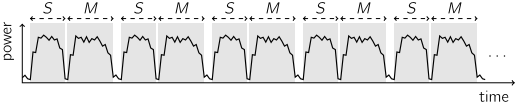
\includegraphics[scale=0.5]{images/SSCA_regular.png}
        \caption{Trace d'un algorithme régulier}
        \label{fig:SSCA_regular}
        \end{figure}
    
    \item[Principes d'atomicité] \hfill \\
    \begin{enumerate}
        \item Formules unifiées : réécrire les formules d'addition et de doublement de telles sortes qu'elles requièrent les mêmes opérations dans le corps de base. Pour certaines formes de courbes, les formules sont naturellement unifiées (voires complètes) : elles s'appliquent que les points en entrées soient identiques ou non. L'attaquant ne pourra plus distinguer quelle opération est effectuée puisque leur consommation électrique sera la même. Il obtiendra une séquence constante d'addition. 
        
        Il est possible de réécrire l'expression du coefficient directeur \footnote{Slope, pente.} $\lambda$ afin qu'il soit valable pour l'addition et le doublement. Les formes Hessiennes ont des formules unifiées assez efficace. Le doublement peut en fait s'écrire comme une addition $[2](X : Y : Z) = (Z : X : Y) + (Y : Z : X)$. Les formes d'Edwards possèdent une arithmétique efficace et intrinsèquement unifiées voire même complète en fonction du paramètre $d$ choisi. 
        
        Notez que cette contre-mesure présente quelques défauts qu'il est important de mentionner :
        \begin{itemize}[label=--]
            \item L'emploie de formules unifiées ne permet pas toujours d'empêcher une SSCA. En effet si l'attaquant est capable d'identifier le passage d'une itération à l'autre, alors il pourra retrouver la séquence d'opération calculée \footnote{En supposant qu'il n'a pas implémenté un algorithme régulier.}. Un bloc constitué de deux opérations représentera un bit égal à $1$. C'est la raison pour laquelle, il est souvent conseillé d'associer des formules unifiées avec un double-and-add atomic. Dans ce cas à chaque itération, une seule opération est effectuée, la consommation électrique de chaque opération se trouve ainsi espacée de manière régulière. 
            \item En supposant que la longueur du scalaire est connue, cette contre-mesure laisse fuir le poids de Hamming de la valeur secrète. En effet le nombre de doublement correspond à la longueur du scalaire et le nombre réel d'addition correspond au poids de Hamming du scalaire. Laisser fuir cette information n'est pas très dangereux et il est possible de masquer le scalaire par des techniques de randomnisation.
        \end{itemize}
        
        \item Atomicité au niveau du corps de base \footnote{Pour ECC mais pas pour RSA.}. L'idée consiste à décomposer l'addition et le doublement en une séquence fixe d'opération dans le corps de base. Cette séquence est appelée un \emph{bloc atomique}. Par exemple une addition peut se calculer par la répétition de $161$ blocs atomiques tandis que le doublement se calcule par une succession de $10$ blocs atomiques. 
        
        Cette contre-mesure présente toutefois deux inconvénients. Le premier est qu'elle remplace les carrés par des multiplications plus coûteuses. Le second est qu'elle introduit des additions, soustractions factices.
        \begin{itemize}[label=--]
            \item Original ECC pattern (Chevallier et al., 03), \cite{chevallier2004low}. 
            \item Longa ECC pattern (Longa, 07), \cite{longa2007accelerating}.
            \item Improved ECC pattern (Girault et Verneuil, 10), \cite{giraud2010atomicity}.
            \item \cite{rondepierre2014revisiting}
        \end{itemize}    
    \end{enumerate}
\end{description}

Il existe des attaques horizontales contres le principe d'atomicité (formules unifiées ou atomicité dans le corps de base) : Big Mac, Big Mac Coco et Horizontal Collision Attacks.


\section{Attaques différentielles par canaux auxiliaires}
\subsection{Présentation}
Une attaque différentielle est mise en place seulement si une attaque simple ne réussit pas. Un attaquant va toujours chercher à s'en prendre aux maillons de sécurité le plus faible. Il testera dans un premier temps, les attaques les plus simples à mettre en oeuvre et augmentera la complexité au fur et à mesure. Pourquoi faire compliquer quand on peut faire simple ?

Les attaques différentielles sont réalisables uniquement lorsque des multiplications scalaires impliquent un même scalaire secret et différents éléments du groupe. Si des multiplications scalaires sont effectuées avec les mêmes éléments, alors on considère la trace moyenne afin d'augmenter les chances de réussite d'une attaque simple. Une DSCA s'attaque par conséquent à la clé secrète de long terme. Les algorithmes ECDSA, ECDHE et ECMQV à deux pas sont naturellement protégés. Ce qui n'est pas le cas pour ECIES. Il faut faire tout de même attention que l'attaquant ne puisse pas récupérer quelques bits de clé secrète éphémère \footnote{Partial key exposure.}, une attaque réseau deviendrait alors possible.

Comme beaucoup d'attaques physiques, les DSCA adoptent le principe de diviser pour régner. On s'attaque à une petite partie de clé, nommée sous-clé. L'attaque est répétée sur chaque sous-clé. Soit l'attaque procède de manière non itérative ce qui est le cas pour les algorithmes symétriques. Soit l'attaque procède de manière itérative, récursive. Dans le premier cas chaque sous clé est indépendante, il est possible de mener ses attaques partielles en parallèles. Tandis que dans le second cas, une partie de la clé doit être découverte afin d'attaquer la suivante.

Il faut collecter un grand nombre de traces (plusieurs milliers) en faisant varier les points (la valeur secrète est fixée). Une matrice de trace est obtenue. Ensuite pour chaque hypothèse de clé, on calcule la valeur intermédiaire théorique associée à la trace. Puis on utilise notre fonction de fuite ou modèle de prédiction afin d'obtenir la matrice de prédictions. Chaque hypothèse faites sur la valeur de la sous-clé, partitionne l'ensemble des traces. Un distingueur est un traitement statistique visant à comparer les valeurs réelles (traces) aux valeurs théoriques (prédictions). Par exemple, on peut employé la moyenne.

Le modèle de fuite crée une sorte de relation d'ordre sur la consommation électrique. En moyenne, la consommation électrique sera différente dans chacune des classes.

\subsection{Contre-mesures}
L'idée consiste à introduire de l'aléa dans le scalaire et dans le point de base. Le mieux est de mettre de l'aléa à la fois dans le scalaire et le point de base.

\begin{description}
    \item[Scalaire] \hfill \\
        \begin{enumerate}
            \item Scalar Randomization. $k^{'} = k + r ord(P)$. Attention la taille du masque doit être suffisamment grande.  
            \item Scalar Splitting. 
                \begin{itemize}[label=--]
                    \item Euclidean Splitting. $k = \lfloor \frac{k}{n} \rfloor + k \pmod r$. Possibilité de faire une multi-exponentation \cite{ciet2003virtually} ainsi le surcoût est faible.
                    \item Additive Splitting. $k = (k + r) - r$ ou $k = k_1 + k_2$. Quelques attaques : Carry Leakage Attack, Combined Attacks. Il est préférable de calculer ces ECSM séparément. 
                    \item Multiplicative Splitting. $k = (k r^{-1}) r$. Deux ECSM sont nécessaires.
                \end{itemize}
            \item Self-Randomized SM.
        \end{enumerate}
     \item[Point de Base] \hfill \\
        \begin{enumerate}
            \item Point Blinding. $[k](P + R)$ et $[k]R$. Tel quelle cette méthode est inefficace mais il existe des variantes moins coûteuses comme l'algorithme BRIP. 
            \item Random Projective Coordinates. \footnote{Also called Coron's 3rd countermeasure.} $[X : Y : Z] = [\lambda X : \lambda Y : \lambda Z]$. Très peux coûteux, mais n'empêche pas les attaques avec les points spéciaux. Il ne faut pas renvoyer le résultat directement en coordonnées homogènes. Il faut soit le convertir en affine et écraser la valeur de $Z$ soit le randomiser à nouveau.
            \item Méthode $2P^*$ de \cite{ciet2003virtually}.
        \end{enumerate}
    \item[Morphisme] \hfill \\
        \begin{enumerate}
            \item Random $E(\field)$ Isomorphism. \footnote{Also called Joye-Timen countermeasure.} $a = -3$ cannot be used.
            \item Random Field \field{} Isomorphism. Special primes cannot be used.
            \item Isogeny Defence. 
        \end{enumerate}
\end{description}

En ce qui concerne le scalaire, on privilégiera clairement la scalar randomization ou bien l'euclidean splitting qui ont des sur-coûts nettement plus faible que les deux autres. 

\section{Attaques par fautes}
\subsection{Présentation}
La première attaque, connue sous le nom d'attaque de Bellcore\footnote{Nom de la compagnie.} due à Boneh et al., remonte à $1997$. Ils injectent une faute durant le calcul d'un RSA-CRT. C'est ensuite au tour de Biham et Shamir d'adapter la technique aux algorithmes symétriques. 

Dans RSA, injecter une faute revient à comparer une signature valide d'une autre invalide. Pour les courbes elliptiques, on vise à injecter une faute dans le point de base, le nombre premier ou la courbe afin que les calculs s'effectue dans une autre courbe que l'on espère faible.

\subsection{Contre-mesures}


\section{Sélection des contre-mesures}
Les contre-mesures à implémenter dépendent à la fois du contexte et du protocole. Les capacités de l'attaquant seront différentes suivants une implémentation sur un serveur web ou sur une carte à puce. Dans le premier temps, on peut considérer que le seul canaux auxiliaires exploitables par un adversaire est le temps. Tandis que pour les cartes à puces, il faudra veiller à se prémunir face à toutes les attaques physiques. 

Le protocole à implémenter joue aussi un rôle prépondérant dans le choix des contre-mesures. Par exemple, le protocole ECDSA est naturellement protégé face aux attaques verticales. L'utilisation de l'échelle de Montgomery permet dans ce cas contre presque toutes les attaques physiques.

Il n'existe pour le moment aucune méthode universelle qui permettrait de se prémunir face à toutes les attaques physiques connues. Il convient donc d'effectuer des choix sur les contre-mesures à implémenter. Ces choix dépendent du contexte de l'implémentation, ils sont donc à faire au cas par cas. En effet une implémentation sur un serveur web sera différente d'une implémentation sur une carte à puce. Dans le premier cas, la plupart des attaques physiques ne sont pas réalisables, alors que pour les cartes à puces c'est une toute autre histoire. De même si mon appareil est conçu uniquement dans le but de signer des messages via ECDSA, je n'aurai à priori pas besoin de me préoccuper des attaques différentielles ou des attaques à la Goubin (puisque l'attaquant ne peut pas choisir le point de base).

Dans tous les cas, trois principes peuvent être retenus pour la sélection d'un ensemble de contre-mesures :
\begin{itemize}
    \item Complet : mon implémentation doit être protégée face à toutes les attaques possibles.
    \item Spécifique : en fonction de l'application, certaines attaques ne s'appliquent pas.
    \item Additif : la combinaison de deux contre-mesures ne doit pas introduire de faiblesse.
\end{itemize}


En plus de se protéger face aux attaques physiques, il est de bon goût de faire une implémentation en temps constant (cf code rules for crypto) : éviter les branchements conditionnels mettant en jeu des données secrètes ... Évidemment cette remarque ne vaut uniquement lorsque l'on est en présence de données sensibles (recodage du scalaire, phase d'évaluation). La phase de pré-calcul peut quant à elle s'implémenter sans soucie de temps constant. L'implémentation de protocoles cryptographiques reste un art délicat dont le moindre écart artistique peut se payer au prix fort et dont l'expérience est un atout indéniable.

\input{10_Security_Requirements.tex}

\chapter{Comptage de points}
Soit $E$ une courbe elliptique définie sur \GF{q} avec $q = p^r$

\begin{description}
    \item[Subfield Curves]\hfill \\
    Soit $\#E(\GF{q}) = q + 1 - a$. \'Ecrivons $X^2 -aX + q = (X - \alpha)(X - \beta)$. Alors
    $$\#E(\GF{q^n}) = q^n + 1 - (\alpha^n + \beta^n)$$
    pour tout $n \geq 1$.
    \item[Symbole de Legendre]\hfill \\
    Pour $x_0 \in \GF{q}$ fixé, le nombre de points de $E(\GF{q})$ d'abscisse $x_0$ dépend si $f(x_0)$ est un carré dans \GF{q} ou non.
    \item[Ordre des points]\hfill \\
    Par le théorème de Hasse, le cardinal des points \GF{q}-rationnels se situe dans un intervalle de longueur $4\sqrt(p) + 1$. La connaissance d'un point de grand ordre permet donc de diminuer l'espace des possibles. L'algorithme BSGS permet de calculer l'ordre du point
    \item[Algorithme de Shoof]\hfill \\
\end{description}

\chapter{Génération d'une courbe elliptique}
Méthode CM \footnote{Multiplication Complexe}, Atkin-Moray sur \GF{p} et Lay-Zimmer sur \GF{2^d}. L'idée est de générer une courbe en spécifiant a priori l'ordre de la courbe. On vise à déterminer une courbe avec un nombre de points donné.

Considérons une courbe elliptique $E$ définie sur l'ensemble des rationnels. En la considérant sur \C, cette courbe possède une multiplication complexe par un ordre dans $\Q(\sqrt{D})$, où $D$ est un entier négatif non carré. Supposons que $p > 3$, un nombre premier ne divisant pas le discriminant de $E$. On peut ainsi considérer $E$ sur \GF{p} en réduisant ses coefficients modulo $p$. Si en plus l'entier est la norme d'un entier algébrique de $\Q(\sqrt{D})$, alors il s'avère que l'on peut facilement calculer le cardinal des points de la courbe $E(\GF{p})$ sans même en connaître ses coefficients, la connaissance des entiers $D$ et $p$ suffit. Le calcul de l'ordre de la courbe peut se faire via l'algorithme de Cornacchia-Smith.

Lié à la théorie des corps quadratiques imaginaires et des formes quadratiques binaires.

La méthode CM est plus rapide que les algorithmes de comptage de points sur une courbe elliptique sur un corps premier ou une extension optimale choisie aléatoirement. Pour les corps binaires, l'utilisation d'algorithme de comptage de points surpasse la méthode CM.

Les utilisateurs ne sont pas confiant quant à l'utilisation de courbes elliptiques en cryptographie générée par la méthode CM. Il est peu probable qu'une courbe sélectionnée au hasard possède un nombre de classe petit. En ce sens, les courbes générées par la méthode CM sont \og spéciales \fg{}. La notion de confiance en cryptographie est fondamentale. On préfère utiliser des courbes plus génériques, qui ne possèdent pas de spécificité. La particularité des courbes CM pourrait être utilisé pour monter une attaque. 

Noter que les courbes CM sont utilisées pour les couplages.


\chapter{ECC security}
\section{Ladders}
Priviligier des algorithmes de multiplication scalaire \emph{régulier}. Le nombre d'opération effectué à chaque itération de la multiplication scalaire est indépendant du scalaire. Peu importe le bit du scalaire considéré, on réalisé autant d'addition que de doublement à chaque pas de l'algorithme. On peut notamment citer : ajout d'opération factices \footnote{dummy operation}, double-and-add always, Montgomery Ladder. Le premier est à é

Priviligier l'utilisation de l'algorithme de l'échelle de Montgomery afin d'effectuer les multiplications scalaires. 

Avantages : simple, rapide (ECSM sans coordonnées $y$ et particulièrement efficace pour les courbes de Montgomery), temps constant.

\section{Twist}
Les attaques suivantes supposent que l'adversaire est en mesure de choisir le point de base de la multiplication scalaire.

\subsection{Attaques de petits sous-groupe}
Attaque de Lim-Lee 1997 \cite{lim1997}. Au lieu d'envoyer un point de la courbe appartenant au sous-groupe principal. On transmet un point de la courbe d'ordre un diviseur du cofacteur. L'ordre de notre point étant choisit petit, on peut ainsi calculer son logarithme discret et par conséquent retrouver le secret modulo l'ordre de notre point. Nous avons ainsi divisé par l'ordre du point le nombre de valeurs possibles restantes pour $k$. 
En pratique cette attaque peut-être ignorée puisque l'attaquant ne récupère que peu d'information sur le secret.

\subparagraph{Contremesures}
\begin{itemize}[label=$\rightarrow$]
    \item Fixer le cofacteur égal à un.
    \item Rejeter les points tel que $hQ = \infini{}$.
\end{itemize}



\subsection{Attaques via courbes invalides}
Attaque présentée en 2000 par Bielh-Meyer-Müller \cite{biehl2000}. L'attaque est basée sur l'observation que les opérations sur les points d'une courbe elliptique (addition et doublement) ne dépendent pas du coefficient $b = a_6$ de la courbe. En d'autres termes, les mêmes formules s'appliquent à l'ensemble des courbes partageant le même coefficient $a = a_2$. 

L'idée consiste à envoyer à Bob un point $Q$ de petit ordre mais appartenant à une autre courbe. En particulier à une courbe de la forme $y^2 = x^3 + ax + c$. D'une part Bob ne se rendra compte de rien s'il ne fait aucune vérification sur le point qu'il reçoit. D'autre part il calculera bien le point $[k]Q$ (et c'est bien ce que recherche Eve).

Ainsi Eve, en récupérant le point $kQ$, peut retrouver un peu d'information sur le secret $k$ : $k \pmod w(Q)$. Il lui suffit de réitérer ce procédé pour un point d'ordre 2, 3, 5 \ldots Dés qu'elle est en possession de suffisamment d'information, elle utilise le CRT pour recouvrer $k$.

Eve doit être capable de construire des courbes dont l'ordre est divisible par de petits entiers et générer des points de petit ordre.

Au final, dés qu'un des coefficients régissant l'équation de la courbe n'intervient pas dans la loi d'addition on peut tenter cette astuce.

\subparagraph{Contremesures}
\begin{itemize}[label=$\rightarrow$]
    \item Vérifier que le point reçu appartient effectivement à la courbe.
    \item Compression des points. En décompressant le point $Q$, Bob s'apercevra automatiquement si le point appartient à la courbe ou non. (Demande du temps et un effort supplémentaire d'implémentation).
\end{itemize}


\subsection{Attaques via courbes invalides contre des ladders}
Cette attaque repose sur le même principe que précédemment. Elle vise les algorithmes d'échelle à une seule coordonnées \footnote{Formules de Montgomery, ou bien les formules de Brier et Joye pour les équations de Weierstrass sur un corps premier.}. 

Commençons par rappeler que l'équation du twist de la courbe elliptique $E : y^2 = x^3 + ax + b$ est donnée par $\tilde{E} : vy^2 = x^3 + ax + b$ où $v$ est un non carré. L'observation clé est que pour ce type de multiplication scalaire, les formules sont les mêmes pour la courbe et son twist. Le coefficient $v$ n'intervient pas. L'attaque consiste donc à transmettre un point du twist qui soit de petit ordre.

\subparagraph{Contremesure}
\begin{itemize}[label=$\rightarrow$]
    \item Vérifier que l'abscisse $x$ correspond bien à un point de la courbe originale et non de son twist.
    \item Twist secure : sélectionner une courbe telle que son twist vérifie les mêmes critères de sécurités que la courbe originalle. Dans ce cas, il n'est plus nécessaire de faire la vérification précédente.
\end{itemize}

Fouque et al. a montré que la première contremesure n'était pas suffisante lorsqu'un attaquant est en mesure de monter une attaque par faute. Par conséquent il est maintenant admis que la notion de twist secure est une propriété attendue d'une courbe elliptique. Il faut bien voir que cette propriété sert uniquement si on implémente un ladder.

Supposons que la vérification se fait après la SM. L'attaquant commence par transmettre un point du twist et de petit ordre. Ensuite juste avant la vérification, il introduit une faute en espérant que le point obtenu passe avec succès le test. Une fois sur deux cela sera le cas. Il obtient le point $[k]P \oplus \epsilon$. Il est raisonnable de supposer que la faute n'a modifié qu'un registre de 8 ou 16 bits. En comparant deux points de cette forme, il peut retrouver $\epsilon$.



\href{http://crypto.stackexchange.com/questions/19878/what-are-these-twist-attacks-with-cost-258-4-on-nist-p-224-curve-and-when}{Lien 1}
\href{http://crypto.stackexchange.com/questions/19877/understanding-twist-security-with-respect-to-short-weierstrass-curves}{Lien 2}

\section{Completeness}
La somme des points d'une courbe elliptique présente des cas particuliers. Il faut vérifier si les points sont identiques, si ils ont la même abscisse \ldots Cette particularité s'avère être un défaut majeur dans la prévention des attaques par canaux auxiliaires. La fuite (la consommation électrique moyenne, le pattern) caractérisant une addition est différente (avec une bonne probabilité) de celle d'un doublement. 

Afin que l'attaquant ne soit plus en mesure de différencier une addition d'un doublement, l'idée consiste à chercher des formules universelles : qui soit applicable à n'importe quelle entrée. On qualifie \emph{d'unifié}, des formules applicables à la fois à l'addition et au doublement. Lorsqu'en plus ces dernières ne présentent plus aucun point particulier, on peut les appliquer à n'importe quel couples de point. On parle alors de formules \emph{complète}. La notion de complétude est donc plus forte (condition suffisante pour être unifié). 



\section{Indistinguishability}



\chapter{Non trié}
\section{Forme de Montgomery 1987}
\begin{definition}
Une courbe elliptique $\mathcal{E} / \GF{p}$ sous forme de Montgomery est donnée sous la forme :
\begin{equation}
By^2 = x^3 + Ax^2 + x =f(x)
\end{equation}
avec $B(A^2 - 4) \neq 0$
\end{definition}
\begin{itemize}[label=$\bullet$]
    \item Symétrique. $-(x, y) = (x, -y)$
    \item Point d'ordre $2$. $2P = \infini{} \Leftrightarrow (x, y) \text{ tel que } y = 0 \text{ et } x \text{ racines de } x(x^2 + Ax + 1)$. En particulier $(0, 0)$ est d'ordre $2$ donc $\# E(\GF{p})$ est pair. Le nombre de points d'ordre $2$ dépend si $A^2-4$ est un résidu quadratique ou non. Ainsi les courbes sous forme de Montgomery sont une sous partie des courbes sous forme de Weierstrass. 
    \item $4 \mid \# E(\GF{p})$. Le cofacteur d'une courbe sous forme de Montgomery vaut au moins $4$.
    \item Arithmétique des courbes sous forme de Montgomery est très efficace. 
    \begin{itemize}[label=--]
        \item La multiplication scalaire s'effectue via le Montgomery Ladder \todo{citer}. Utiliser tel quel cet algorithme est intéressant car c'est un algorithme régulier, ce qui le rend immunisé face aux attaques temporelles. \'{A} chaque itération, qu'importe la valeur du bit considéré une addition et un doublement est effectué. Le nombre d'additions et de doublements dépend de la longueur de la chaîne de bits. Mais il ne dépend pas du bit pattern ni de la valeur des bits. De plus le nombre d'opération dans le corps fini est identique.
        \item D'autre part, il est possible de se limiter à la première coordonnée. Il devient ainsi plus efficace que les algorithmes d'exponentiation traditionnels. Pour cela, il faut montrer que connaissant $x(nP)$ on peut retrouver $y(nP)$. Et que l'on peut calculer $x(2P)$ et $x(P+Q)$ connaissant $x(P), x(Q), x(P-Q), y(P-Q)$.
        \item Le doublement implique une multiplication par $\frac{A \pm 2}{4}$. On choisit le coefficient $A$ tel que cet entier soit petit.
    \end{itemize}
    \item Lopez et Dahab ont généralisé la technique en $99$ aux courbes binaires et Brier et Joye en 2002 l'ont étendu aux formes de Weierstrass sur un corps premier mais le nombre de multiplications pour l'addition et le doublement est moins intéressant pour les courbes de Montgomery. 
    \item Transformation sous forme de Weierstass et vice-versa. 
    \item Avantages : immunisé naturellement contre les attaques temporelles et l'arithmétique est très efficace.
    \item Curve25519 : créer par Bernstein pour un ECDH.
    \item Les courbes de Montgomery sont redoutables pour les multiplications scalaires simples mais elles sont moins adaptées pour les multiplications scalaires multiples.
    \item Elles sont birationnnelement équivalentes aux twist des courbes d'Edwards.
\end{itemize}

Quelques papiers notables :
\begin{itemize}[label=--]
    \item \href{http://sage.math.washington.edu/edu/124/misc/montgomery.pdf}{Papier de Montgomery}
    \item \href{http://saluc.engr.uconn.edu/refs/sidechannel/okeya00elliptic.pdf}{Elliptic curves with their Montgomery form}. Apporte des conditions nécessaires et suffisantes pour l'existence de point d'ordre $4$, $8$.
    \item \href{http://cr.yp.to/ecdh/diffchain-20060219.pdf}{Chaîne d'addition différentielle de Bernstein 2006}.
    \item \href{https://eprint.iacr.org/2006/220.pdf}{Chaîne d'addition multidimensionel pour les courbes de Montgomery 2006}.
\end{itemize}

\section{Forme d'Edwards}
\subsection{Sur un corps NON binaire}
\begin{itemize}[label=--]
    \item Le théorème suivant établit que toutes les courbes elliptiques définies sur un corps non binaire sont birationnellement équivalentes à une forme d'Edwards sur une extension du corps de base. En effet toutes courbes elliptiques possèdent un point d'ordre $4$ dans une extension.
    \begin{theoreme}
    Soit \field{} un corps tel que $2 \neq 0$. Soit $E$ une courbe elliptique définie sur \field{} possédant un point \field{}-rationnel d'ordre $4$. Alors :
    \begin{enumerate}
        \item Le twist quadratique de $E$ est birationnellement équivalent sur \field{} à une forme d'Edwards.
        \item Si en plus $E(\field{})$ possède un unique point d'ordre $2$ alors le coefficient $d$ est un non carré. Ce qui implique que les formules d'additions sont complètes.
        \item Si en plus \field{} est fini, alors $E$ est birationnellement équivalent sur \field{} à une forme d'Edwards. 
    \end{enumerate}
    \end{theoreme}
    \item Soit $E : x^2 + y^2 = 1 + dx^2y^2$, une courbe d'Edwards sur un corps \field{} non binaire tel que $d \neq 0, 1$. On définit la loi d'addition comme :
    $$ (x_1, y_1), (x_2, y_2) \mapsto \left ( \frac{x_1y_2 + x_2y_1}{1 + dx_1x_2y_1y_2}, \frac{y_1y_2 - x_1x_2}{1 - dx_1x_2y_1y_2} \right )$$
    Cette opération définit bien une loi de composition interne. L'élément neutre est le point affine  $(0, 1)$. L'opposé d'un point $P$ est donné par $-P = (-x_1, y_1)$. De plus $(0, -c)$ est d'ordre $2$ et $(c, 0)$, $(-c, 0)$ sont d'ordres $4$.
    \item Cette opération de groupe est \emph{fortement unifiée} : elle est aussi définie pour le doublement de points. Il existe cependant quelques cas où l'addition n'est pas définie : le dénominateur s'annule. On peut montrer que cette situation n'arrive jamais lorsque $d$ est un non carré. Dans ce cas on dit que la loi est \emph{complète} : l'opération est définie pour toutes les paires de points de la courbe.
    \item DBL : 3M + 4S = 6,2M. ADD : 10M + 1S. Le gain est important par rapport à une forme de Weierstrass : 1S pour le DBL et 1M + 4S pour l'ADD. Les formes d'Edwards présentent un doublement compétitif et l'une des additions les plus efficaces.
    \item Au final quelque soit la configuration, multiplication scalaire simple ou multiple avec ou sans contremesure, la forme d'Edwards sur un corps non binaires possèdent l'arithmétique la plus efficace. Cependant elle reste concurrencée par les courbes de Montgomery pour la SM simple et par les courbes à multiplication complexe (courbes de Koblitz et courbes GLV). On peut aussi rajouter les quartiques de Jacobi.
    \item Introduction du \emph{système de coordonnée inversé}. Il permet de gagner une multiplication sur l'addition sans réduire l'efficacité du doublement et du triplement. Néanmoins les formules ne sont plus complètes mais uniquement fortement unifiées. Les points spéciaux restent limités : points d'ordres $2$, $4$ et le point à l'infini.
\end{itemize}

\noindent Listes de papiers notables :
\begin{itemize}[label=--]
    \item \href{http://citeseerx.ist.psu.edu/viewdoc/summary?doi=10.1.1.139.567}{A normal form for elliptic curve. Edwards 2007}.
    \item \href{http://cr.yp.to/newelliptic/newelliptic-20070906.pdf}{Faster addition and doubling on EC 2007.}
    \item \href{http://eprint.iacr.org/2007/410.pdf}{Inverted Edwards coordinates 2007}.
    \item \href{http://eprint.iacr.org/2008/013.pdf}{Twisted Edwards Curves}.
    \item \href{http://eprint.iacr.org/2008/522.pdf}{Twisted Edwards Curves Revisited}.
\end{itemize}

\subsection{Sur un corps binaire}
\begin{definition}
Soit \field{} un corps tel que $char(\field{}) = 2$. Soient $d_1, d_2 \in \field{}$ tel que $d_1 \neq 0$ et $d_2^2 \neq d_1^2 + d_1$. L'équation affine d'une coubre d'Edwards binaire est donné par :
$$E_{B, d_1, d_2} : d_1(x+y) + d_2(x^2 + y^2) = xy + xy(x + y) + x^2y^2$$
L'équation est symétrique en $x$ et en $y$ donc si $(x_1, y_1) \in E_{B, d_1, d_2}$ alors $(y_1, x_1)$ est aussi un point de la courbe. $e = (0, 0)$, $T_2 = (1, 1)$ et $(x_1, y_1) + (1, 1) = (x_1 + 1, y_1 +1)$.
\end{definition}

\begin{itemize}[label=--]
    \item La loi d'addition est fortement unifiée : la formule peut aussi être utilisée pour le doublement, mais il existe quelques cas exceptionnel. Lorsque le paramètre $d_1 \neq 0$ et qu'il n'existe aucun élément $t \in \field{}$ satisfaisant $t^2 + t + d_2 = 0$ ou de manière équivalente lorsque $k = \field{2^n}$ $d_2$ vérifie $Tr(d_2) = 1$, alors la loi d'addition est complète (les fonctions rationnelles définissant l'addition n'ont aucun pôle sur $E_{B, d_1, d_2}$).
    \item Si $n \geq 3$, alors toutes les courbes elliptiques sur \GF{2^n} sont birationnellement équivalentes à une courbe d'Edwards binaire complète.
\end{itemize}



\section{Courbes elliptiques définies sur un corps binaire}
Nous considérons ici les courbes elliptiques définies sur \GF{2^d}. 
\begin{equation}
\left (\frac{\delta f}{\delta x}(P); \frac{\delta f}{\delta y}(P) \right) = (a_1 y + x^2 + a_4; a_1 x + a_3)
\end{equation}
On peut transformer l'équation de Weierstrass en fonction de la valeur de $a_1$.

\paragraph{Courbe supersingulière}
Si $a_1 = 0$, alors $a_3 \neq 0$. Sinon elle n'est pas lisse. 
\begin{equation}
E : y^2 + a_3y = x^3 + a_4x + a_6
\end{equation}
Rappelons que $-P = (x, - a_1x - a_3 - y)$. Ainsi $2P = \infini{} \Leftrightarrow a_3 = 0$. On a donc $E[2] = \{\infini{}\}$. C'est une courbe supersingulière. Utilisé pour les couplages.

\paragraph{Courbe ordinaire}
Si $a_1 \neq 0$, on peut transformer l'équation de Weierstrass en :
\begin{equation}
E : y^2 + xy = x^3 + a_2x^2 + a_6
\end{equation}
Cette courbe est lisse (ie : elle définit une courbe elliptique) si et seulement si $a_6 \neq 0$
\begin{itemize}[label=$\bullet$]
    \item $E[2] = \{ \infini{}, (0, \sqrt{a_6})\} \subseteq E(\GF{2^d}) \implies E(\GF{2^d})$ est d'ordre pair. Par définition une courbe ordinaire possède un point d'ordre $p$, la question est de savoir à quelle extension appartient-il ?
    \item En pratique $d$ est impair.
    \item Lorsque $d$ est impair, il est toujours possible de choisir $a_2 \in \GF{2}$. S'il existe $\lambda \in \GF{2^d}$ tel que $\lambda^2 + \lambda + c = 0$ avec $c \in \GF{2^d}$. Alors le changement de variable suivant
    \begin{equation*}
    x \mapsto x, y \mapsto y + \lambda x
    \end{equation*}
    conduit à l'équation de Weierstrass 
    \begin{equation}
    y^2 + xy = x^3 + (a_2 + c)x^2 + a_6
    \label{EC_binaire}
    \end{equation}
    On peut montrer que $\lambda$ existe si et seulement si $Tr_{\GF{2^d}/\GF{2}}(c) = 0$. Ainsi on cherche $c$ de trace nulle et tel que $a_2 + c \in \GF{2}$. Il suffit de prendre $c$ égal à $a_2$ ou $a_2 + 1$. Lorsque $d$ est impair, l'un de ces éléments est de trace nulle ($Tr_{\GF{2^d}/\GF{2}}(1) = d$).
    \item Il est possible d'accélérer le doublement en coordonnée affine lorsque on peut déterminer les solutions des polynômes de degré 2. Ce qui est le cas en représentation normale.
    \item Lorsque l'on a plusieurs doublement consécutifs à effectuer en affine. On accélère les calculs en représentant les points par leur abscisse et la pente de la tangente.
    \item Lopez et Dahab ont généralisé l'idée de Montgomery en 99. On peut appliquer l'échelle de Montgomery uniquement en calculant les abscisses des points.
    \item Point Halving.
    \item Compression. Il y a au plus deux points avec la même abscisse $(x,y)$ et $(x,x+y)$. On représente un point par $x$ et un bit. L'équation \eqref{EC_binaire} a deux solutions dans \GF{2^d}. On pose $Y = y / x$. L'équation devient $Y^2 + Y + (x^3 + a_2x^2 + a_6)/x^2$. Cette dernière a une solution si et seulement la trace du terme constant est nulle. Les solutions sont alors $Y$ et $Y+1$. Le bit du poids faible de $y/x$ permet de distinguer les solutions. Problème la compression est coûteuse, nécessite une inversion.
\end{itemize}

\subsection{Point Halving}
Technique proposé de indépendamment par Knudsen et Schroeppel en 99. Elle permet de calculer plus efficacement la multiplication scalaire en substituant les doublements par l'opération halving (moitié). Cette technique est applicable uniquement pour les courbes elliptiques binaires de cardinal divisible par $2$ mais pas par $4$ (ce qui est équivalent à $Tr(a_2) = 1$).

$\# E(\GF{2^d}) = 2^k l$, où $l$ est impair. On dit que $E$ est en $2$-torsion minimal \footnote{$E$ is said to have minimal $2$-torsion.} si $k=1$. 

Considérons l'endomorphisme de doublement :
$$\fonction{[2]}{E(\GF{2^d})}{E(\GF{2^d})}{P}{[2]P}$$
C'est un morphisme non injectif $Ker([2]) = E[2] = \{ \infini{}, T_2\}$. Chaque point possède exactement $2$ antécédents ($A$ et $A + T_2$).
On a : $E(\GF{2^d}) = G \times E[2^k]$. On peut définir l'application réciproque du doublement sur $G$.
$$\fonction{[\frac{1}{2}]}{G}{G}{P}{Q \hspace{1cm} [2]Q = P}$$
$[\frac{1}{2^i}] := [\frac{1}{2}] \circ \ldots [\frac{1}{2}]$

\begin{itemize}[label=$\bullet$]
    \item $E$ sur $\GF{2^d}$ est en minimal $2$-torsion $\Leftrightarrow Tr_{\GF{2^d}/\GF{2}}(a_2) = 1$
    \item Comment représenter un entier par son développement $\frac{1}{2}$-adic.
    \item Comment calculer l'opération halving. Chaque point possède exactement deux antécédents par $\frac{1}{2}$. Il faut être capable de distinguer $[\frac{1}{2}]P$ de $[\frac{1}{2}]P + T_2$. Lorsque $k=1$ on peut le faire facilement en remarquant que l'on peut calculer la moitié de $[\frac{1}{2}]P$ mais pas de $[\frac{1}{2}]P + T_2$. 
    \item Le calcul de la moitié d'un point demande de calculer efficacement les racines carrés et de résoudre des équations du second degré.
    \end{itemize}
    Lorsque $k=1$, l'application halving est facilement calculable et est notamment plus rapide que le doublement. On peut ainsi substituer le doublement par l'opération halving et rendre la multiplication scalaire plus efficace.


\subsection{Courbes de Koblitz}
Koblitz a proposé en $92$ l'utilisation en cryptographie des courbes définies sur \GF{2}. On les appelle les courbes de Koblitz ou encore les courbes anomales binaires\footnote{Les courbes de Koblitz sont anomales sur \GF{2} ou son twist est anomale toujours sur \GF{2}.}. Avec ces courbes, il est possible de substituer le doublement par le Frobenius. Mais pour que cela soit intéressant il faut vérifier plusieurs choses : que l'évaluation du Frobenius soit rapide, que le développement $\tau$-adic s'effectue rapidement et que ce développement soit court et creux (faible densité). Le premier limite le nombre d'évaluation du Frobenius tandis que le second influence le nombre d'addition.

L'utilisation d'un endomorphisme est à mettre en parallèle avec les techniques de recodage du scalaire. La dernière vise à diminuer le nombre d'addition tandis que la première cherche à réduire le coût des doublements, en les substituant par un endomorphisme. 
\begin{equation}
E_a / \GF{2} : y^2 + xy = x^3 + a_2x^2 + 1
\end{equation}

\begin{itemize}[label=$\bullet$]
    \item $E_1$ est anomale sur \GF{2} mais pas forcément sur \GF{2^d}. Le twist de la courbe $E_0$ est anomale sur \GF{2}.
    \item  $\# E_{a_2}(\GF{2}) = 3 - \mu = 3 - (-1)^{1-a_2}  = \begin{cases} 2 & \text{ pour } a_2 = 1 \\ 4 & \text{ pour } a_2 = 0\end{cases}$.\\
    Le cofacteur $h$ de $E(\GF{2^d})$ est au moins divisible par $2$. En pratique, on le choisira minimal. Soit $h = 2 $ ou $4 = 3 - (-1)^{1-a_2} = 3 - \mu = (\tau - 1)(\bar{\tau} - 1)$
    \item Spécifier une courbe de Koblitz, revient à définir un nombre premier $d$. Si l'on considère les nombres premiers compris entre $160$ et $512$, il existe seulement $12$ courbes de Koblitz intéressantes pour la cryptographie.  
    \item On peut facilement calculer $\# E(\GF{2^d})$ à partir de $\# E(\GF{2})$ via les suites de Lucas. On note $\tau$ et $\hat{\tau}$ les racines du polynômes caractéristiques de Weil. On a les relations suivantes : $\tau \hat{\tau} = 2$ et $\tau + \hat{\tau} = \mu$. On identifie le Frobenius au nombre complexe $\tau$. 
    \item Les courbes de Koblitz ont été introduites car en partie leurs normes et leurs traces sont petits. L'endomorphisme de Frobenius \footnote{Dans ce contexte, on l'appelle squaring map.} vérifie l'équation : $\tau^2 + 2 = \mu \tau$ avec $\mu = (-1)^{1-a_2}$. Cet endormorphisme est quasiment gratuit à calculer. 
    \item Cette application peut être vue comme implémentant la multiplication complexe par $\tau = \frac{\mu + \sqrt{-7}}{2}$. On a $X^2 - \mu X + 2 = (X - \tau)(X - \bar{\tau})$. D'où $\tau \bar{\tau} = 2$ et $\tau + \bar{\tau} = \mu$.
    \item Pour calculer ECSM, on regarde l'entier $k$ comme un élément de $\Z[\tau]$. Par exemple pour $a = 1$ \footnote{On parle de la trace.}, on a $9 = \tau^5 - \tau^3 +1$. En considérant le calcul de $\tau$ comme gratuit. Une ECSM correspond ici à $3$ additions. C'est donc le poids de Hamming du développement de $k$ qui détermine le coût ie : le nombre d'addition.
    \item $\Z[\tau]$ est un anneau euclidien par rapport à la fonction norme, $N(z) = z \bar{z}$. Toutefois la propriété d'être euclidien, n'affirme pas l'unicité du quotient et du reste mais seulement de leurs existences. L'algorithme de division usuel consiste à choisir le reste minimisant la norme du quotient. Pour le développement $\tau$-adic NAF, lorsque $n_0$ est impair, on sélectionnera le reste tel que le quotient soit divisible par $\tau$.
    \item Développement $\tau$-adic. Soit $k \in \Z[\tau]$, on définit 
    \begin{equation*}
        k = \sum_{i = 0}^{l-1} k_i \tau^i
    \end{equation*}
    avec $k_i \in \{0, 1 \}$ pour tout $0 \leq i \leq l-1$.
    \item Développement $\tau$-adic en forme non adjacente (NAF). Même chose sauf que $k_i \in \{0, \pm 1\}$ et vérifie la propriété de non adjacence : pour tout couples de bits consécutifs au moins un est nul. $k_i k_{i+1} = 0$, pour tout $0 \leq i \leq l-2$.
    \begin{itemize}[label=--]
        \item Pour chaque élément de l'anneau $\Z[\tau]$, la représentation $\tau$-adic NAF est unique.
        \item Le nombre de coefficient non nul (qu'on appelle souvent la densité) dans le développement $\tau$-adic NAF est minimal parmi les représentations à valeurs dans $\{0, \pm1\}$. La densité est égal à $1/3$.
    \end{itemize}
    
    \item Le développement \og standard \fg{} $\tau$-adic d'un scalaire aléatoire est de longueur $2\log{n}$ et de densité égale à $1/3$. Ce phénomène d'expansion est fâcheux, le coût d'une ECSM passe donc en moyenne de $2\log{n}$ Frobenius et $2/3\log{n}$ Add à $\log{n}$ Dbl et $\log{n}/3$ Add. Le gain ne s'avère donc pas aussi grand qu'espéré. 
    
    \item Pour un même niveau de sécurité, à cause des frobenius, il faut ajouter quelques bits.
    
    \item Pour un niveau de sécurité qui nous intéresse, soit entre $80$ et $350$, il existe seulement $14$ courbes de Koblitz vérifiant les critères de sécurité attendus (avec en particulier un cofacteur minimal). Allez lire le post \href{http://crypto.stackexchange.com/questions/10263/should-we-trust-the-nist-recommended-ecc-parameters}{Should trust the NIST ?}.
\end{itemize}


\section{Courbes DIK}
DIK 

% Pour compiler :
% :!pdflatex main.tex; makeindex main.nlo -s nomencl.ist -o main.nls; pdflatex main.tex;


\section{Kangaroo in SCA}
\begin{itemize}[label=--]
    \item Présentation d'une nouvelle technique d'énumération de clé. Appliqué à la cryptographie asymétrique et plus précisément à courbes elliptiques. Utilise des informations partielles issues d'une attaque template de la multiplication scalaire lors d'un échange de clé de DH. Les techniques d'énumération de clé existant ne sont pas applicables dans ce contexte car ici les bits de clé ne sont pas indépendant. 
    \item L'attaque se déroule en deux phases :
    \begin{description}
        \item[Phase d'élimination ou de sélection.] Une attaque template sur la multiplication scalaire lors d'un DH est réalisée. Les résultats de cette attaque correspondent à la donnée des probabilités à posteriori : probabilité 
    \end{description}Dans un premier une phase d'élimination ou de sélection. Via une attaque template, on récupère les probabilités à posteriori 
\end{itemize}

\begin{comment}
\section{A faire}
\begin{itemize}
    \item Degré de plongement d'une courbe elliptique.
\end{itemize}

\begin{definition}
    Soit $E(\GF{q})$ une courbe elliptique et $r$ un diviseur premier de $\# E(\GF{q})$. Le \emph{degré de plongement} de $E$ relativement à $r$ est le plus petit entier $k$ tel que $r|q^k - 1$
\end{definition}
\end{comment}

\section{Résumé : exigences de sécurité}
\subsection{Sécurité DLP}
\begin{itemize}[label=$\bullet$]
    \item Attaques génériques sur le logarithme discret. 
    \begin{itemize}[label=$\rightarrow$]
        \item Algorithme de Silver-Pholig-Hellman : la complexité du DLP dépend du plus grand nombre premier divisant l'ordre du de $g$. Si cet entier lisse (composé de petits facteurs premier) alors le DLP est facile. Ainsi l'ordre de $g$ doit contenir un grand nombre premier pour éviter cet attaque. De plus si l'ordre de $g$ contient de petit facteur, il est possible de retrouver de l'information partielle sur le log discret. 
        \item La méthode Rho de Pollard casse ECDLP en utilisant en moyenne $\sqrt{\pi l / 4} = 0.886 \sqrt{l}$ additions. Ainsi si on souhaite atteindre un niveau de sécurité de $n$ bits, il faut que $l$ soit de taille $2n$. Safecurves exige $100$ bits de sécurité. C'est un algorithme probabiliste il peut donc terminer plus tôt (ou plus tard), en particulier sa probabilité de succès après $m$ additions est de $m^2 / l$. De plus casser plusieurs DLP en même temps n'est pas équivalent à les casser individuellment. Il y a un effet racine carrée.
    \end{itemize}
    \item Transfert du ECDLP
    \begin{itemize}[label=$\rightarrow$]
        \item Attaque du à Smart qui permet de transférer le problème du logarithme discret dans le groupe additif d'un corps fini. Il faut vérifier que la courbe n'est pas anomale : $\# E(\GF{p}) \neq p$.
        \item S'assurer que le degré de plongement $k$ de $l$ soit petit. Les standards SECG et ANSI X9.62 exige que $k$ soit supérieur à 20. IEEE P1363 demande que $k$ soit supérieur à 30. Enfin Brainpool et Safecurves préconise que $k$ soit supérieur à $(l-1)/100$. Rappelons que $k$ par rapport à $l$ est défini comme étant le plus entier naturel tel quel $l | q^k - 1$. Cette exigence permet de se prémunir contre l'attaque MOV et l'attaque Frey-Rück.
    \end{itemize}
    \item Discriminant de la multiplication complexe
\end{itemize}

\subsection{Sécurité SCA}
\begin{itemize}[label=$\bullet$]
    \item 
\end{itemize}

\subsection{Efficacité}
\begin{itemize}[label=$\bullet$]
    \item Choix d'une courbe tel (ou via isomorphisme) $a_2 = -3$
    \item Forme spéciale du modulo $p$. L'entier $p$ est un nombre de Crandall ie : un polynôme ternaire évalué en une puissance de 2 ou un nombre pseudo-Mersenne. Recommandé par le NIST et SECG. Tandis que le standard Brainpool exige que l'entier $p$ ne doit posséder aucune forme spécifique.
    \item Choisir $p$ tel que $p \equiv 3 \pmod 4$. On transmet $(x, LSB(y))$, puis on retrouve $y$ via $(x^3 +ax + b)^(\frac{p+1}{4}) = y y^{\frac{p-1}{2}} = \pm y$.
    \item 
\end{itemize}

\subsection{Compression}
Les protocoles cryptographiques nécessitent souvent l'envoie d'un point d'une courbe elliptique à travers un canal. Pour un corps premier de $200$ bits (soit $25$ octets), un point est représenté par $50$ octets. Si la bande passante est un critère important, il est possible de la diminuer en utilisant la technique de \emph{compression d'un point}. Si $q$ est codé sur $n$ bits, alors il est possible de représenter un point d'une courbe par $n+1$ bits au lieu de $2n$ bits. On distingue le cas d'un corps fini binaire ou non. Soit $P = (x, y)$ un point de la courbe $E$.
\begin{itemize}
    \item Corps fini non binaire. On a $\GF{p^d} = \GF{p}(\theta)$, où $\theta$ est un élément primitif. $y = \sum_{i = 0}^{d-1} y_i \theta^i$. On peut représenter le point $P$ par $(x, LSB(y_0))$. On retrouve $y^2$ avec la connaissance de $x$ et on obtient $\pm y$. Il est possible de distinguer ces deux valeurs\footnote{Qui correspondent à un point et à son opposé.} en remarquant que $y_0$ et $-y_0 = -y_0 + p$ sont de parités différentes. La décompression nécessite deux multiplications et le calcul d'une racine carrée (via algorithme de Tonelli-Shanks).  Si $p \equiv 3 \pmod 4$, ce qui est préconisé par le nouveau standard de Brainpool, il est alors possible de décompresser le point sans calculer une racine carrée via l'égalité : $(y^2)^{(p+1)/4} = y y^{(p-1)/2}$.
    \item Corps binaire. Encore la même question : connaissant l'abscisse d'un point de la courbe, quelles informations avons-nous besoin afin de récupérer son ordonnée ? En divisant par $x_1^2$, et en posant $z = y /x_1$, on obtient l'équation $z^2 + z +(x^3 + a_2x^2 + a_6)/x^2 = 0$ qui admet une solution si et seulement si la trace du terme constant est nul. Si $z$ est une solution alors l'autre est $z + 1$ \footnote{De même si P est sur la courbe alors $-P = (x, x+y)$ aussi.}. On représente un point par $(x, LSB(y/x))$. La compression, contrairement à un corps non premier, nécessite une inversion. La décompression requiert de résoudre une équation, de distinguer la bonne solution et de multiplier par $x$ pour retrouver $y$. Il existe une technique pour représenter un point avec $n-1$ bits au lieu de $n+1$ \href{http://citeseerx.ist.psu.edu/viewdoc/download;jsessionid=FCE13676C67E9FD34EF1BDDE6D898011?doi=10.1.1.26.4672&rep=rep1&type=pdf}{[ici]}.
    \item Courbes de Koblitz. Ce n'est pas une technique de compression à proprement parler, puisque l'on ne peut pas recouvrer le point de manière certaine. C'est une technique permettant de réduire le nombre de bits à transmettre pendant le protocole d'échange de clé de DH. Utilise les classes d'équivalence modulo le Frobenius ou de manière équivalente modulo une rotation. 
\end{itemize}

Il est d'usage durant la phase d'implémentation de coder le point à l'infini comme $(0, 0)$. Afin d'éviter toute ambiguïté, le standard Brainpool préconise que le paramètre $b$ soit un non résidu quadratique dan \GF{p}. Dans le cas contraire la représentation des points compressés de $(0, 0)$ et de $(0, X)$, où $X = LSB(b)$, serait identique.

\section{Utilisation d'endomorphisme}
Afin d'accélérer la multiplication scalaire, il peut être intéressant d'utiliser des endomorphismes facilement calculable. Une idée naturelle est de voir ce qu'il est possible de faire avec le Frobenius. Cette application étant à égal à l'identité sur les points définis dans le corps de base, elle n'a donc d'intérêt seulement pour des courbes sur corps non premiers\footnote{donc binaire}. Remarquons tout de suite que son évaluation correspond à un décalage à gauche en représentation normale et nécessite au plus trois carrés en représentation polynomiale. Son polynôme caractéristique est de la forme $X^2 - aX + q$, on peut ainsi naturellement substituer la multiplication scalaire par $q$ par une addition et deux Frobenius. 

En 90, Menezes et Vanstone ont proposé d'appliquer cette idée à une courbe binaire avec une trace nulle. Cela conduisait à substituer l'opération de doublement par le Frobenius. Malheureusement cette courbe est supersingulière et l'on sait depuis 93 que cette famille de courbes est faible.

En 92, Koblitz a suggéré d'utiliser les deux courbes non supersingulières sur \GF{2} restantes. On parle des courbes de Koblitz ou encore aussi appelé courbes anomales binaires. Solinas en 99 a nommé ces courbes ainsi car une des deux courbes de Koblitz est anomale sur \GF{2} tandis que pour la seconde, c'est son twist qui est anomale \GF{2}. Bien entendu, ces courbes ne sont pas anomales sur $\GF{2^d}$. Le développement $\tau$-adic d'un entier s'effectue de la même façon que le développement binaire. Au lieu de diviser par $2$, on divise par $\tau$. De même on calcul le $\tau$-NAF suivant le même principe que le 2-NAF. Si n est divisible par $\tau$\footnote{En notant $n = c_0 + \tau c_1$, ceci est équivalent à $c_0$ est pair.}, alors le bit vaut 0 et on enchaîne avec $n/\tau$. Si n n'est pas divisible par $\tau$ cette fois, alors on choisit la valeur du bit $\epsilon = \pm 1$ de tel sorte qu'il respecte la propriété de non-adjacence. C'est à dire que $(n - \epsilon)/\tau$ soit divisible par $\tau$ ou autrement dit que $n - \epsilon$ soit divisible par $\tau^2$ \footnote{Ce qui peut se vérifier facilement.}. 
Cependant pour qu'un développement d'un entier soit intéressant il faut qu'il soit à la fois court et creux. Court afin de diminuer le nombre d'évaluation de l'endomorphisme et creux \footnote{Assurer par la propriété de non adjacence.} pour diminuer le nombre d'addition. Le développement présenté plus haut est de longueur de $2\log{n}$ et de densité $1/3$. On passe donc de $\log{n}$ DBL et $\log{n}/3$ ADD à $2\log{n}$ Frob et $\log{n}2/3$ ADD. Le gain n'est pas aussi grand qu'espérer. Mais il est possible d'éviter ce phénomène d'expansion. 

\section{CoZADD}
En 2007 Méloni a proposé une formule d'addition de points partageant la même coordonnée en $Z$ en coordonnées Jacobienne. Puisqu'elle demande des conditions particulières sur les opérandes, il est logique qu'elle soit plus efficace que tout autres formules d'addition. Ce qui l'est moins, c'est qu'elle surpasse aussi les formules de doublement proposées jusqu'ici.

Muni de cette nouvelle addition, on aimerait bien pouvoir l'employer dans une multiplication scalaire. L'observation clé est que son addition fournit implicitement un représentant d'une des opérandes partageant la même coordonnée en $Z$ que le résultat de l'addition. Via une chaîne d'addition adaptée\footnote{Appelée chaîne d'addition euclidienne.}, il devient maintenant envisageable de calculer une multiplication scalaire avec ces formules. De plus on peut se limiter aux coordonnées $(X_3, Y_3)$ puisque $Z$ n'intervient pas. Comme pour l'échelle de Montgomery on retrouve $Z$ et donc $Z_3$ à la fin.

Les chaînes d'addition sont de la forme $v = (1, 2, 3, v_4, \ldots, v_s)$. Pour être utilisable avec les formules de Méloni, il faut que les opérandes des additions induient pour la chaîne d'addition partagent la même coordonnée en $Z$. Ainsi à chaque itération, seuls deux possibilités s'offrent à nous. Par exemple prenons $(1, 2, 3, 4)$. On a $3 = 2 + 1$. Pour le suivant on a seulement le choix entre $3 + 2$ et $3 + 1$. Et ainsi de suite.

Les suites de Fibonacci sont des chaînes d'addition euclidiennes optimales. Méloni a tenté d'utiliser la représentation de Zeckendorf : écrire un entier comme la somme de nombres de Fibonacci. Finalement il propose un Fibonacci-and-add efficace mais légèrement plus lent que son homologue binaire. 

Combine les additions coZ avec les algorithmes de types échelles. Pour cela, ils remarquent qu'avec un surcoût de $1M + 1S$ l'addition coZ permet aussi calculer la différence. On est ainsi en possession des deux algorithmes efficaces suivants : 
$(P_1 + P_2, \tilde{P_1} \leftarrow coZADDU(P_1, P_2)$ et $(P_1 + P_2, P_1 - P_2) \leftarrow coZADDC(P_1, P_2)$.
L'échelle de Montgomery calcul : $R_{1-b} \leftarrow R_{1-b} + R_b$; $R_b \leftarrow 2R_b$. 
Qui peut se réécrire sous la forme : 
$T \leftarrow R_{b} - R_{1-b}$; $R_{1-b} \leftarrow R_{1-b} + R_b$
$R_{1-b} \leftarrow R_{1-b} + T$
Ce qui correspond à un coZADDU suivit d'un coZADDC.

Au final on obtient une nouvelle version du Montgomery Ladder nommée $(X, Y)$-only coZ Montgomery Ladder. Légèrement plus efficace que la version x-only d'une courbe de Weierstrass, elle présente en plus l'avantage d'être naturellement immunisée face à l'attaque par faute de Fouque.


\section{Critères sélection de nouvelles courbes}
Différentes parties ont donné leur point de vue concernant la confiance (ou non) entourant les courbes standardisées, en fonction des propriétés qu'elles satisfont ou non, ou du procéder pour les générer. 

%%%%%%%%%%%%%%%%%%%%%%%
% BIBLIOOGRAPHY
%%%%%%%%%%%%%%%%%%%%%%%
% Citer un article : \cite{etiquette}
\bibliographystyle{plain}             % plain, alpha, unsrt, abbrv
\bibliography{notes.bib}               % affiche seulement les références cités
%\nocite{*} ou \nocite{ref}           % fait apparaitre la ref sans l'avoir cité 
          

                 
\end{document}